\documentclass{article}
\usepackage[utf8]{inputenc}
\usepackage{graphicx}
\usepackage{subcaption}
\usepackage{listings}
\usepackage{color}
\usepackage{pdflscape}
\usepackage{float}
\usepackage{comment}
\usepackage{mathtools}
\usepackage{rotating}
\usepackage{tikz}
\usepackage{csquotes}

\definecolor{dkgreen}{rgb}{0,0.6,0}
\definecolor{gray}{rgb}{0.5,0.5,0.5}
\definecolor{mauve}{rgb}{0.58,0,0.82}

\DeclarePairedDelimiter\ceil{\lceil}{\rceil}

\lstset{frame=tb,
  language=C++,
  aboveskip=3mm,
  belowskip=3mm,
  showstringspaces=false,
  columns=flexible,
  basicstyle={\small\ttfamily},
  numbers=none,
  numberstyle=\tiny\color{gray},
  keywordstyle=\color{blue},
  commentstyle=\color{dkgreen},
  stringstyle=\color{mauve},
  breaklines=true,
  breakatwhitespace=true,
  tabsize=3
}


\title{CS-531 \\
        PA 3: Sudoku}
\author{Tommy Hollenberg \\
        Matthew Phillips \\
        Michael Slater}
\date{February 20, 2019}

\begin{document}

\maketitle

\begin{abstract}
        \noindent This document describes experiments solving Sudoku puzzles using backtracking search with constraint propagation. Different sets of inference rules are applied when solving the puzzles and the puzzle difficulty is judged based upon the inference rules used to find the solution. The effectiveness of the most-constrained variable heuristic versus a fixed baseline is also examined. 
\end{abstract}
\clearpage

\pagenumbering{arabic}
\tableofcontents
\clearpage
\section{Introduction}
Sudoku is a puzzle game played on a 9x9 grid. The initial state of the grid is mostly blank cells with a few cells containing values. The goal of the game is to fill each cell with a digit ranging from one through nine so that the values in each row or column satisfy the \textsc{All-Diff} constraint. Also, the grid is sub divided into nine 3x3 blocks. Each solved puzzle's 3x3 blocks' values must satisfy the \textsc{All-Diff} constraint. The \textsc{All-Diff} constraint demands that each value in a row, column, or block is distinct.

Our Sudoku solver uses backtracking search applying inference rules to reduce variable domains. This is an application of constraint satisfaction problem solving. We will compare the efficacy of different inference rule sets and variable selection heuristics in terms of minimizing the amount of guessing needed for a solution.
\section{Backtracking Search}

Backtracking search was used to solve the puzzles. First, the inference rules in the inference scheme (discussed below) are applied repeatedly to restrict the variable domains until none can be applied. If applying the inference rules brings some variable domain down to a single value, that value is assigned to that variable, and constraints are propagated before continuing inference rule applications. If an unassigned variable domain becomes empty, then we must backtrack, because some of the constraints have been violated. After inference is complete, we check whether a solution has been found. If not, a guess must be made. The question of which variable to guess a value for is decided by one of two heuristics, which are discussed below. Then, one of the remaining values in the selected variable domain is assigned. If the guess does not create a conflict (by restricting some other unassigned variable's domain to zero elements), then the backtracking search is called recursively on the new board state.

If the recursive call does not find a solution, then the guess and all associated domain restrictions are undone, and the next value in the variable's domain is tried. If none of the values in the domain yields a solution, then a bad guess has been made higher up the recursive stack, so we return failure to backtrack further.

\noindent\makebox[\linewidth]{\rule{\columnwidth}{0.4pt}}
\emph{backtracking search pseudocode}\\
backtrackingSearch (grid)\\
\indent if(grid.inference()==fail)\\
\indent \indent return false\\
\indent if(grid.complete())\\
\indent \indent return true\\
\indent domain=grid.getDomain(variables)\\
\indent for value in domain\\
\indent \indent grid.newLayer()\\
\indent \indent if(grid.guessCount()$>$1000)\\
\indent \indent \indent return true\\
\indent \indent if(grid.guess(val, var) and backtrackingSearch(grid))\\
\indent \indent \indent return true\\
\indent \indent grid.backtrack()\\
\indent return false\\
\noindent\makebox[\linewidth]{\rule{\columnwidth}{0.4pt}}
\subsection{Inference Rules}
Backtracking search implementing Sudoku inference rules is a form of forward checking. Each inference rule may constrain the domain of the grid variables or assign a value to a variable if it is the only value remaining in the domain. Forward checking reduces future value conflicts between variables and therefore reduces backtracking. 

Each inference rule is derived from the \textsc{All-Diff} constraint of each row, column, and block of the grid.
\subsubsection{Naked Single}
If there is only one remaining value in a cell's domain, assign that value to that cell. 
\subsubsection{Hidden Single}
if there is a value in a cell's domain that is not in any other cell's domain of that row, column, or block, assign that value to that cell.
\subsubsection{Naked Pair}
An identical pair that occurs in a row, column, or box. Remove it from other rows, columns or blocks that share both these cells.
\subsubsection{Hidden Pair}
A pair of numbers that occurs only in two cells in a row, column, or box. Eliminate the other numbers from them.
\subsubsection{Naked Triple}
Three numbers that do not have any other numbers residing in the cells with them. Eliminate them from the rest of the cells in the same row, column, or box. 
\subsubsection{Hidden Triple}
Similar to hidden pairs, but three numbers instead.
\subsection{Heuristics}
After the inference rules can no longer either assign values or additionally restrict domains, the search must guess the next value assigned. Two different heuristics were used in our backtracking search. 
\subsubsection{Fixed Ordering}
The fixed ordering heuristic assigns values to cells in a left to right fashion, beginning with the top row and continuing onto the next highest row after each row is filled. The smallest value from a cell's domain is selected first. If the smallest value fails, the next smallest value is selected and so on.
\subsubsection{Most Constrained Variable}
The most constrained variable heuristic searches the grid for the cell with the least remaining values in its domain. If there is a tie between two or more cells, the first cell encountered in the search is kept. The grid is searched in a left to right fashion, starting with the top row and continuing with the next highest row and so on. The smallest value in the most constrained cell's domain is assigned. If that value fails the next smallest value is assigned and so on.
\section{Experimental Setup}
The file provided with the assignment description contained 77 puzzles ranked from Easy to Evil. All 77 puzzles were solved using each of the two heuristic (fixed ordering, most-restricted variable), and with four different sets of inference rules (no inference, naked/hidden singles only, naked/hidden singles and pairs, naked/hidden singles, pairs, and triples). The number of guesses made and the number of applications of each specific inference rule were tracked for each solution attempt. If the puzzle was not solved in 1000 guesses, the search was stopped, and the number of squares filled at that point was recorded.

\section{Results}
Each team should try to solve all the problems, starting with the easy ones. Report the number of problems solved and the number of backtracks with each problem. Experts appear to grade the problems by the complexity of rules needed to solve them without backtracking. Is this conjecture roughly correct? Grade each problem, by the set of rules used in solving it. Report also the average number of filled-in numbers (in the beginning) for each of these types of problems. Would this accurately reflect the difficulty of the problem?

Report your results in the form of a mini-paper as you did for the other two assignments. Give the pseudocode for the algorithm. Discuss how the results vary with the difficulty of the problems, and the effectiveness of the most-constrained variable heuristic compared to fixed selection. Also report on the effectiveness of rule subsets in reducing the search. Is the number of backtracks reduced by increased inference rules? Please feel free to include any other observations.

\subsection{Puzzles Solved and Timing}
There were a total of 616 total puzzle configurations tested. This reflects 8 different configurations for each of 77 puzzles. Out of these 616 total puzzles, 602 puzzles were solved within the experiment 1000 step limit. The average number of backtracking steps to complete these solved puzzles vs. the expert rated difficulty of the puzzles is shown in figure \ref{fig:avg_steps_solved_puzzles}.

\begin{figure}[H]%
	\centering\begin{tabular}{c}
		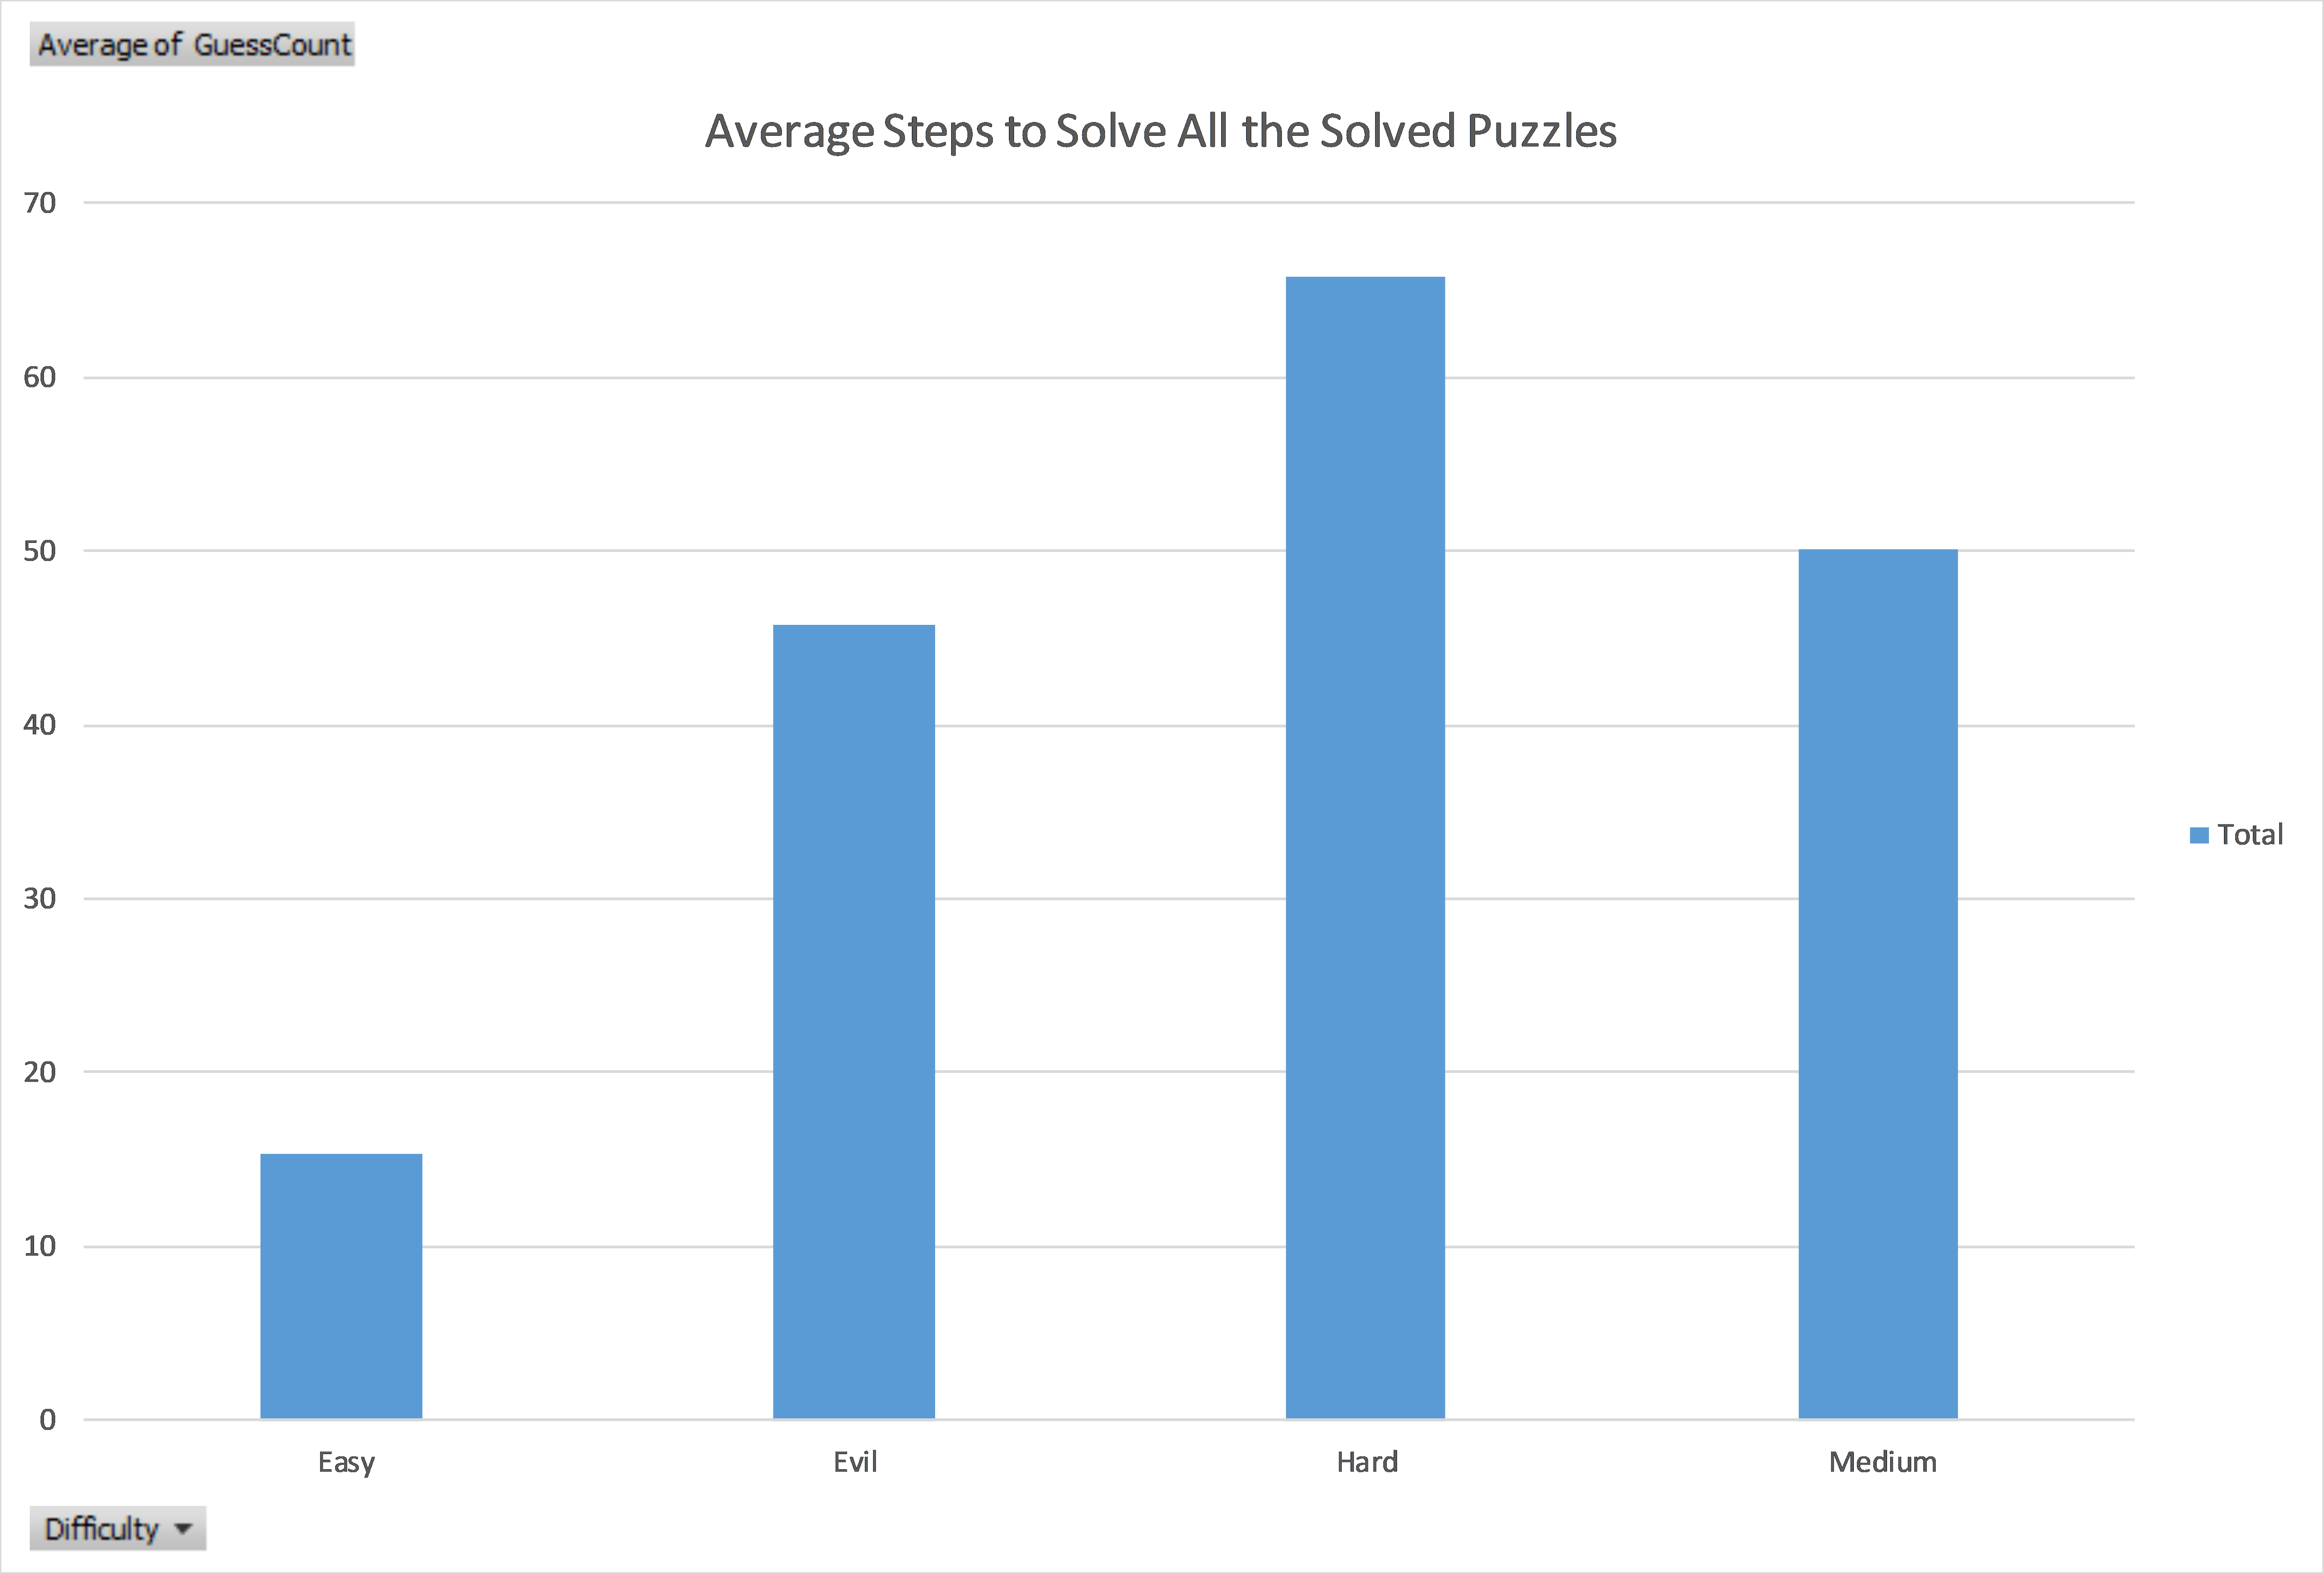
\includegraphics[scale=0.5]{plots/avg-steps-solved-puzzles.png}\\
	\end{tabular}
	\caption{Average Steps To Solve The Solved Puzzles}%
	\label{fig:avg_steps_solved_puzzles}%
\end{figure}

Beyond the solved puzzles, there were 14 puzzles that could not be solved within 1000 steps. All of these puzzle configurations did not use the MRV heuristic to pick a cell. The distribution of these unsolved puzzles across the expert puzzle difficulties is shown in figure \ref{fig:dist_unsolved_vs_diff}.\\

\begin{figure}[H]%
	\centering\begin{tabular}{c}
		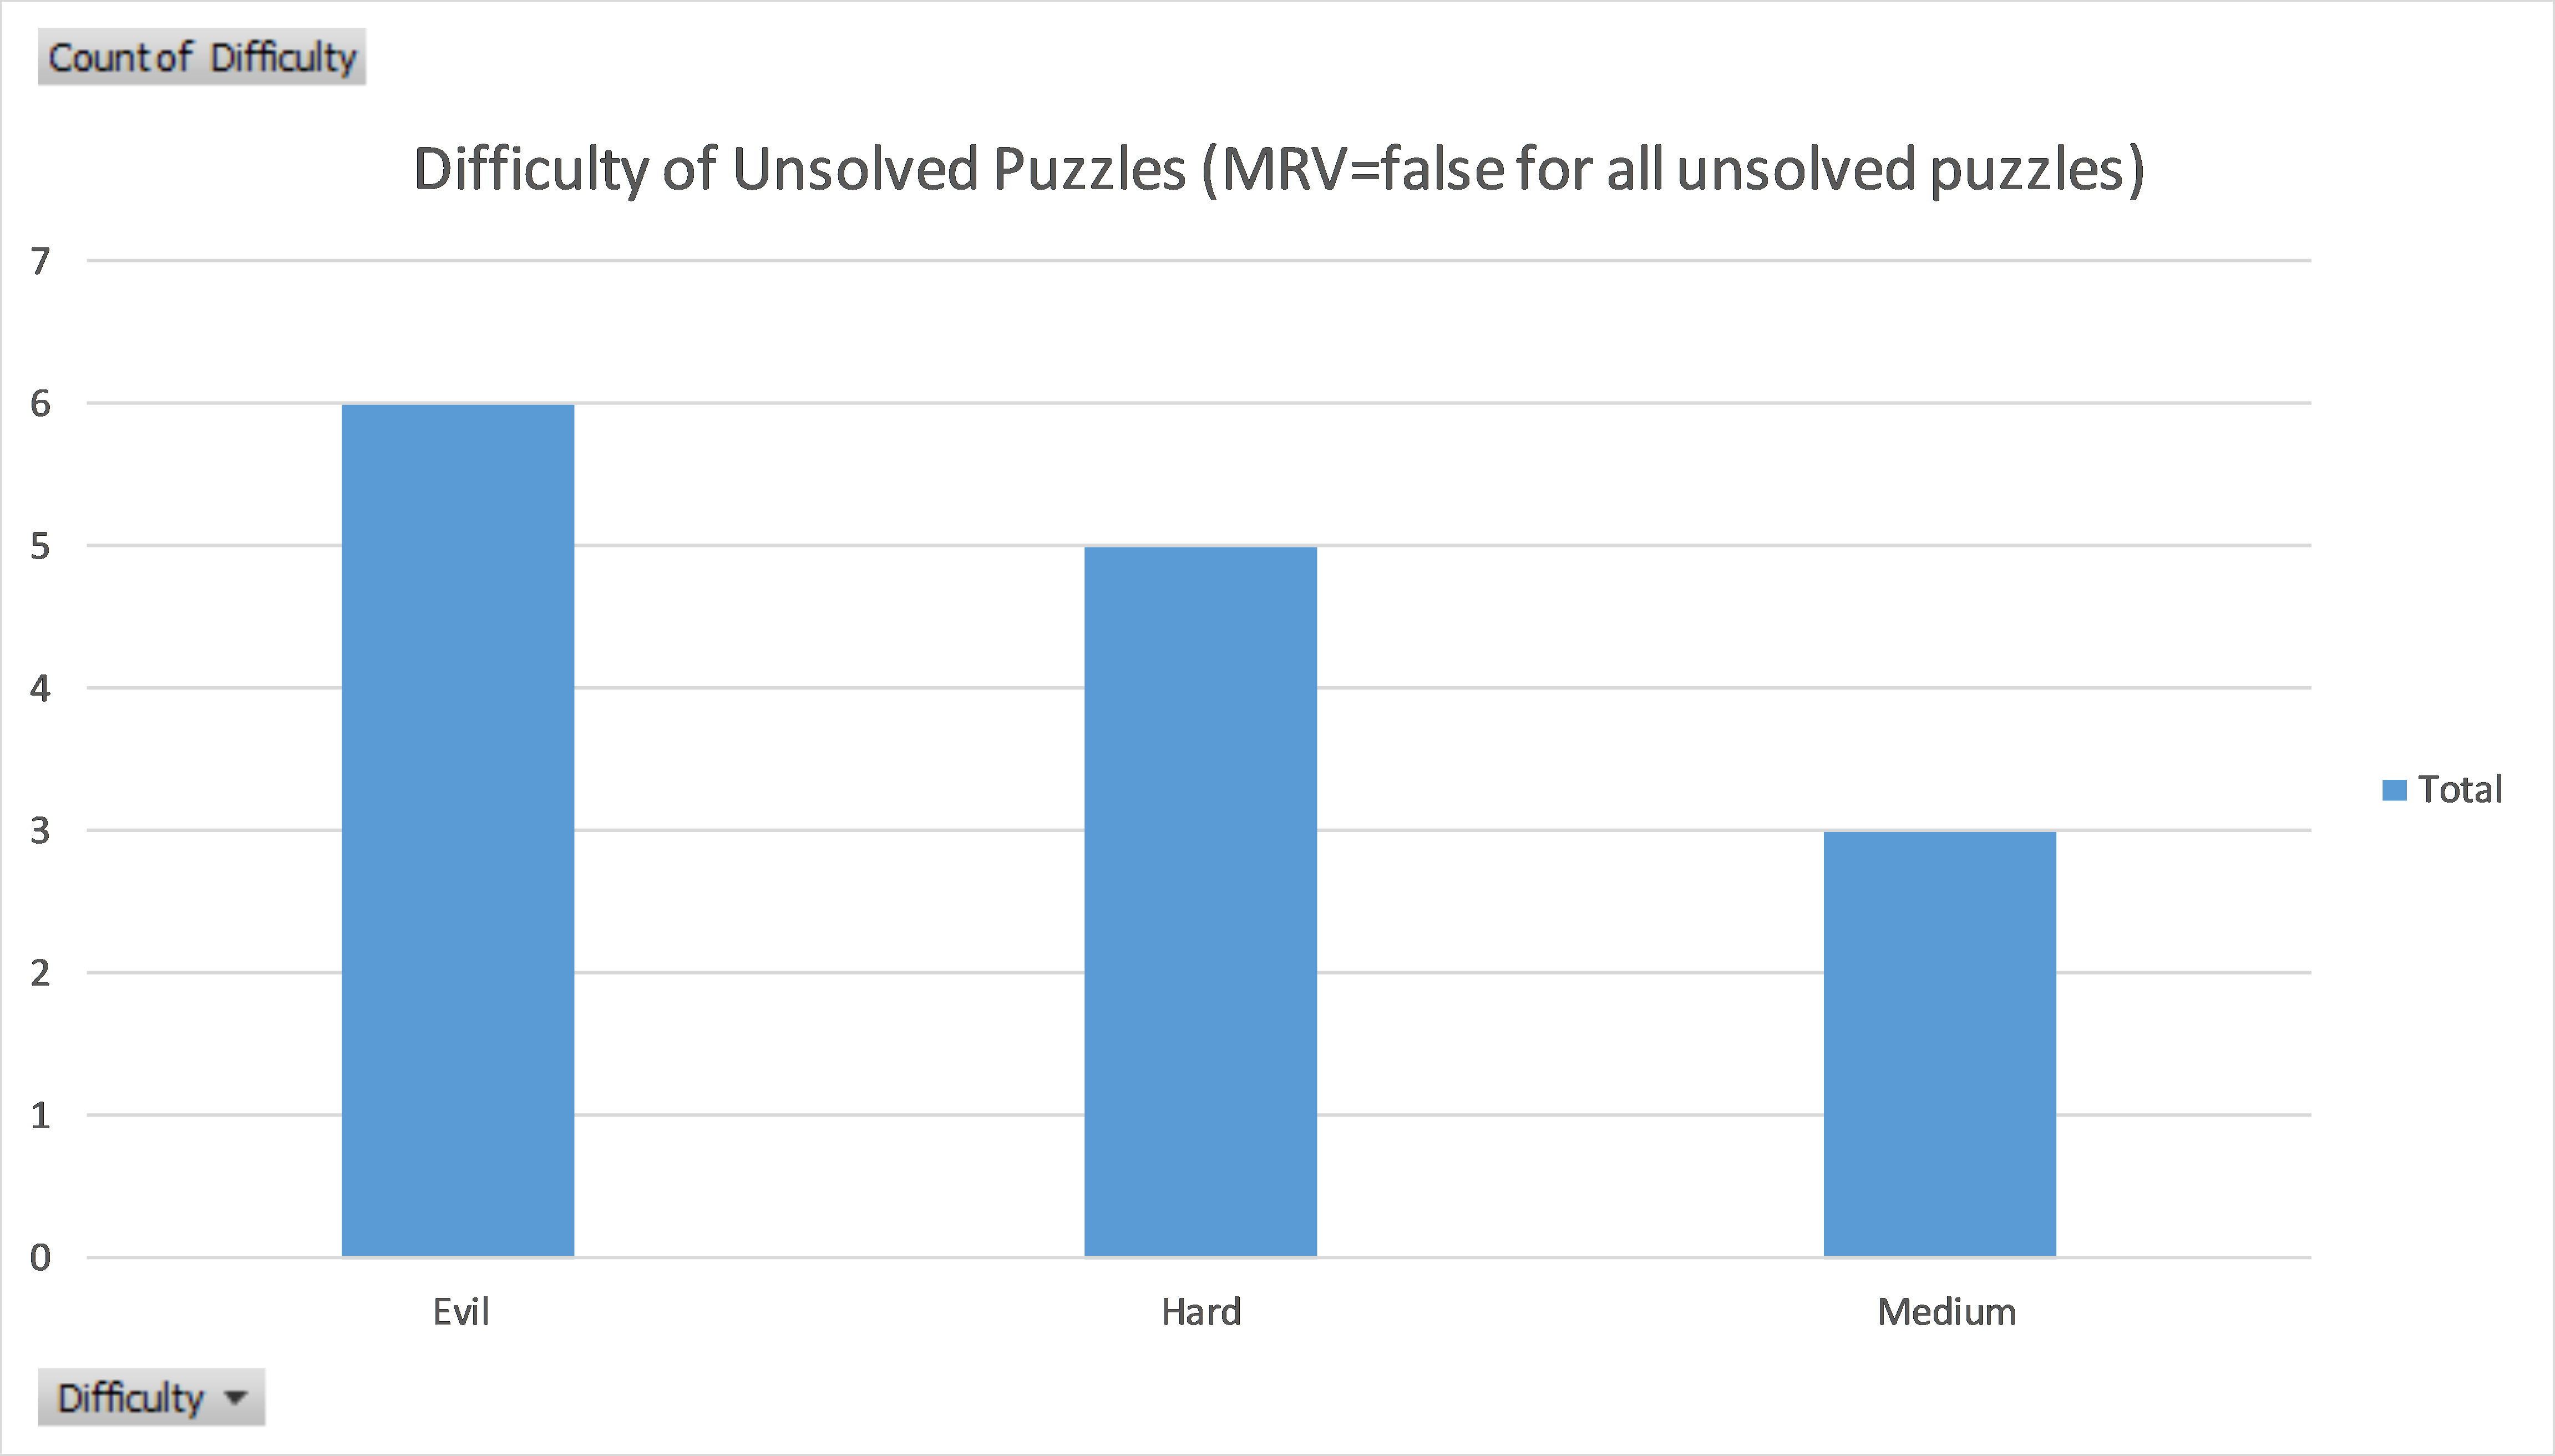
\includegraphics[scale=0.5]{plots/count-unsolved-puzzles-vs-expert-diff.png}\\
	\end{tabular}
	\caption{Distribution of Unsolved Puzzles vs. Expert Difficulty}%
	\label{fig:dist_unsolved_vs_diff}%
\end{figure}

The total time spent on all puzzle solving for the 616 puzzle configurations was approximately 670 milliseconds. The average puzzle solving time is just under 1.1 millisecond per puzzle and is shown in table \ref{table:puzzle_timing}.\\

\begin{table}[h!]
	\begin{center}
		\caption{Puzzle Solving Time}
		\label{table:puzzle_timing}
		\begin{tabular}{|c|c|}
			\hline 
			Total experiment time & 669.912	milliseconds \\ 
			\hline 
			Total puzzles & 616 \\ 
			\hline 
			Average puzzle time & 1.087519481 milliseconds \\ 
			\hline 
		\end{tabular}
	\end{center}
\end{table}

\subsection{Difficulty, Inference Scheme, Inference Heuristics}
The amount of backtracking spent on each puzzle was greatly dependent on how a cell was picked, e.g. using the fixed baseline or using the MRV heuristic. The total and average backtrack counts versus the cell-picking method can be seen in in figure \ref{fig:total_backtracks_vs_mrv_heuristic} and figure \ref{fig:avg_backtrack_count_vs_cell_heuristic}, respectively.\\

\begin{figure}[H]%
	\centering\begin{tabular}{c}
		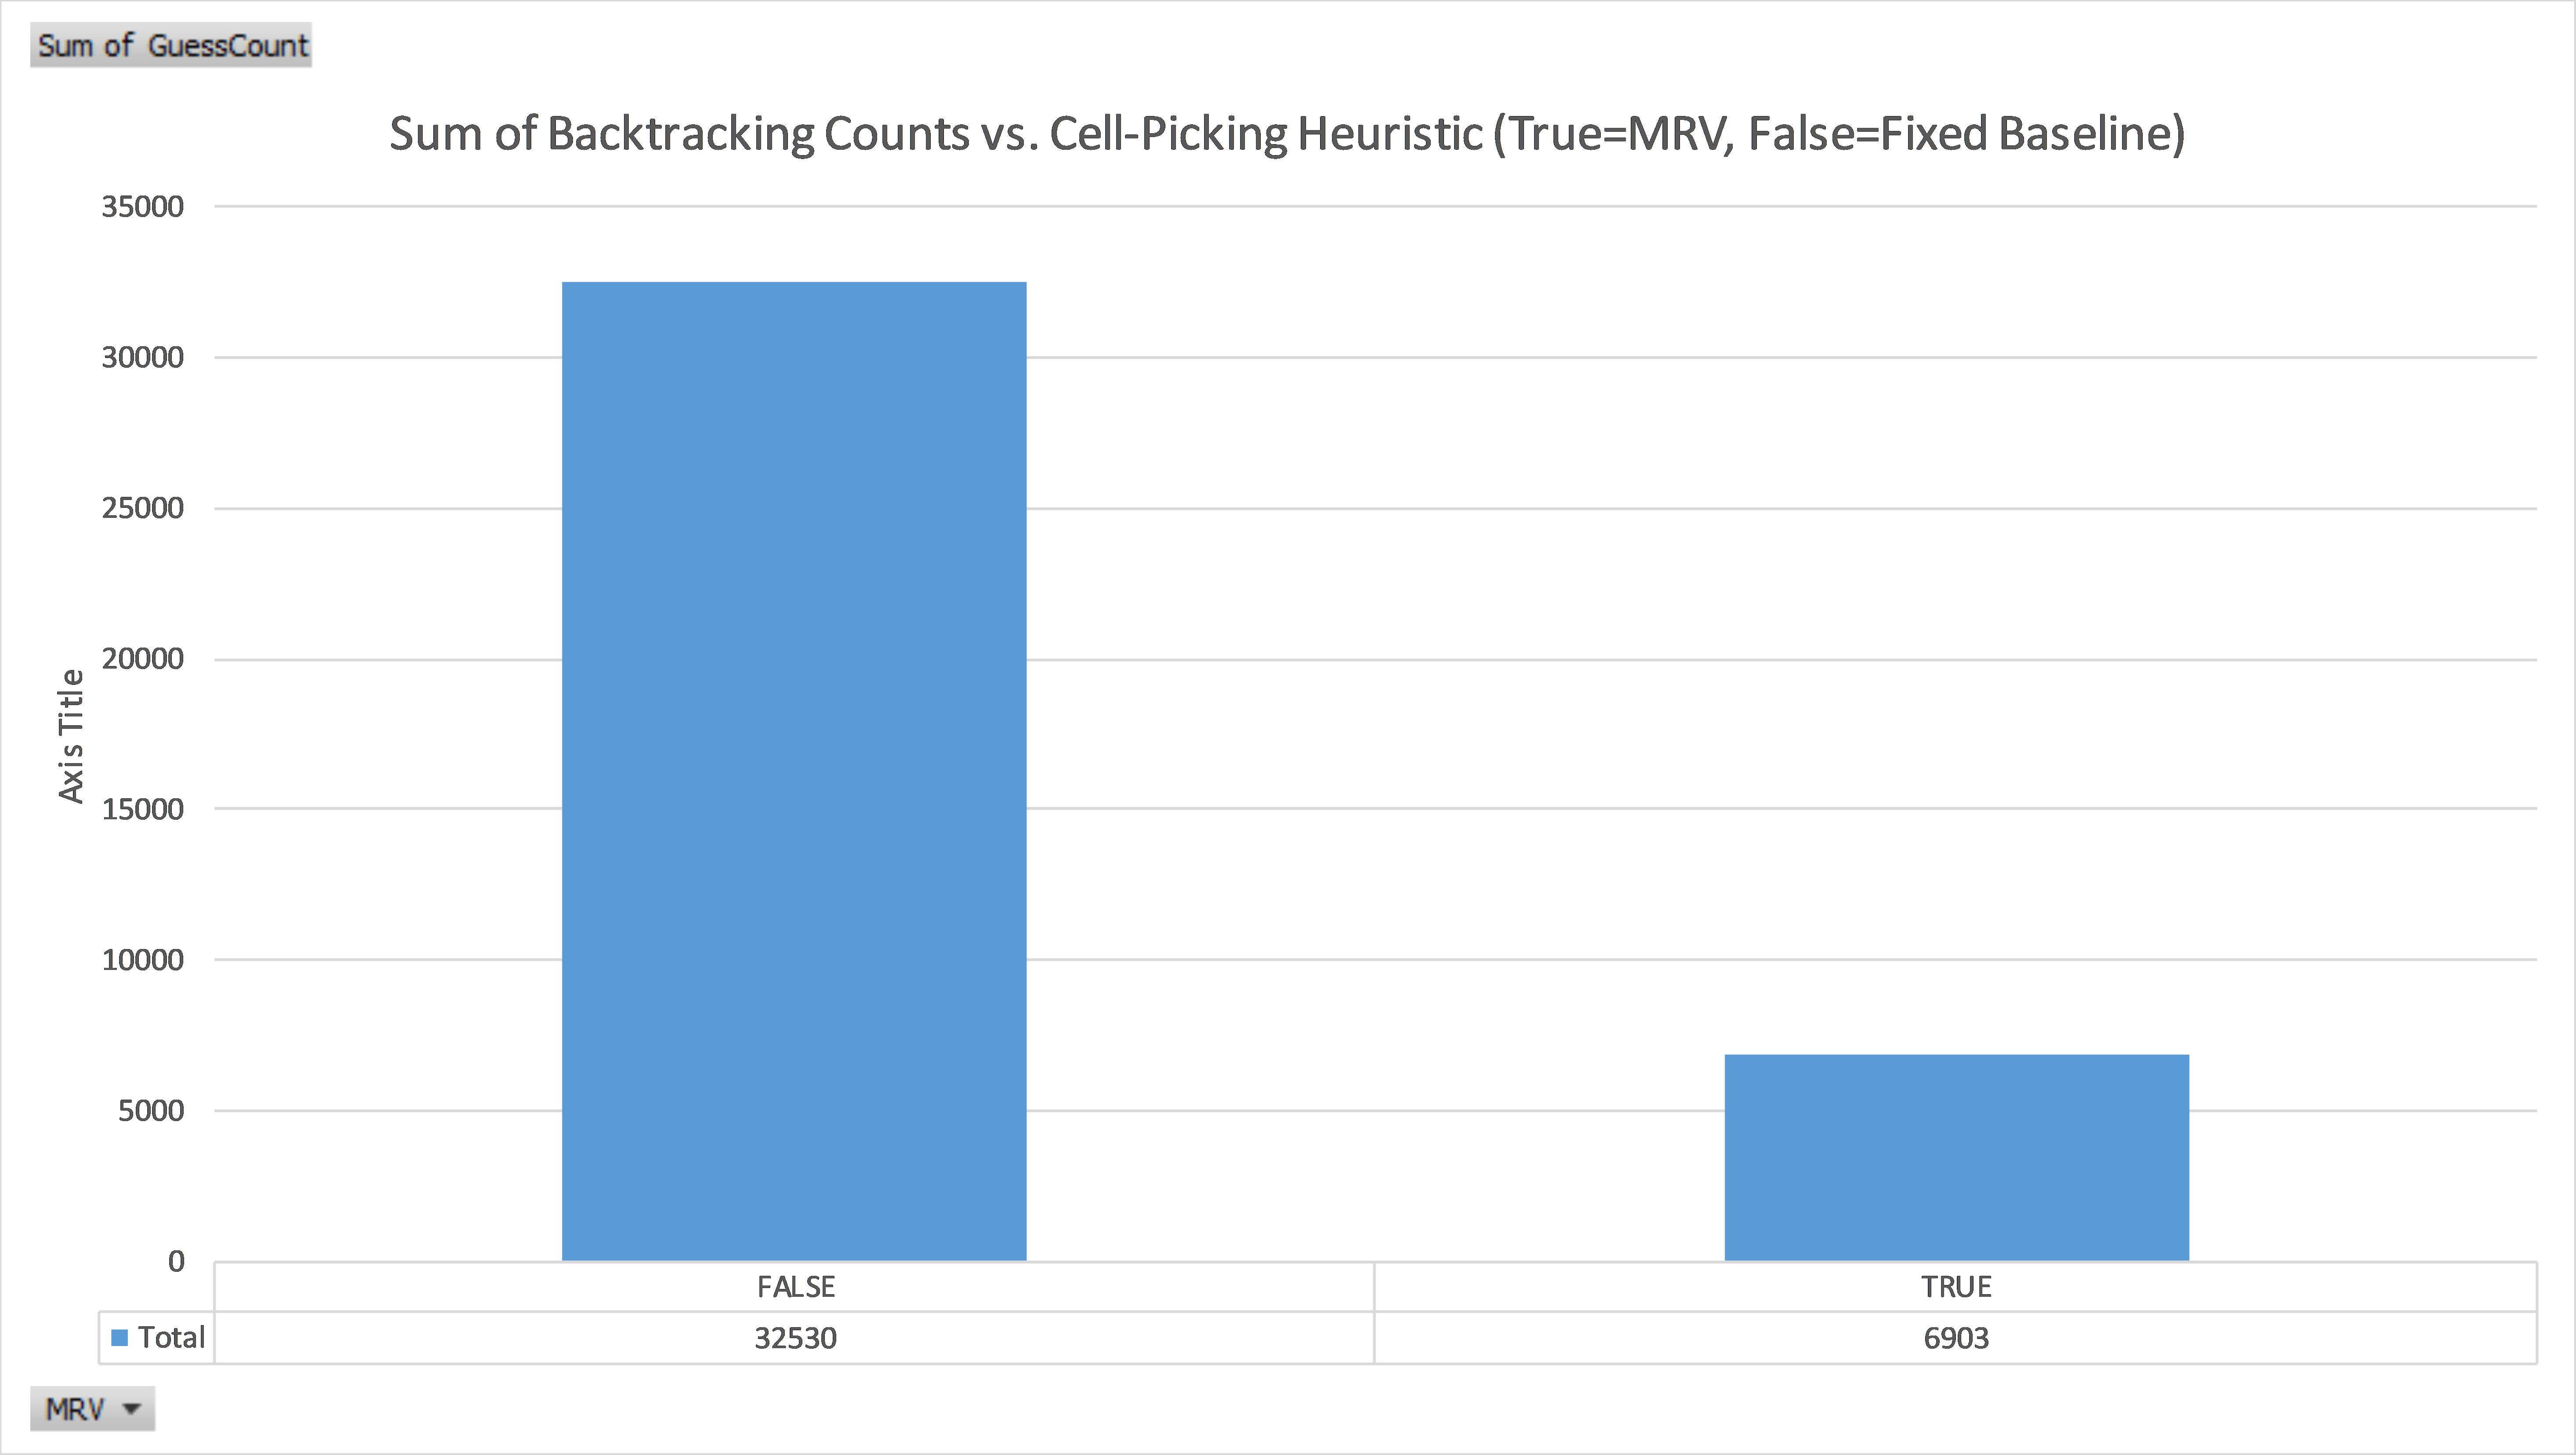
\includegraphics[scale=0.4]{plots/sum-backtrack-count-vs-cell-picking-heuristic.png}\\
	\end{tabular}
	\caption{Total Backtrack Count vs. Cell-Picking Heuristic}%
	\label{fig:sum_backtrack_count_vs_cell_heuristic}%
\end{figure}

\begin{figure}[H]%
	\centering\begin{tabular}{c}
		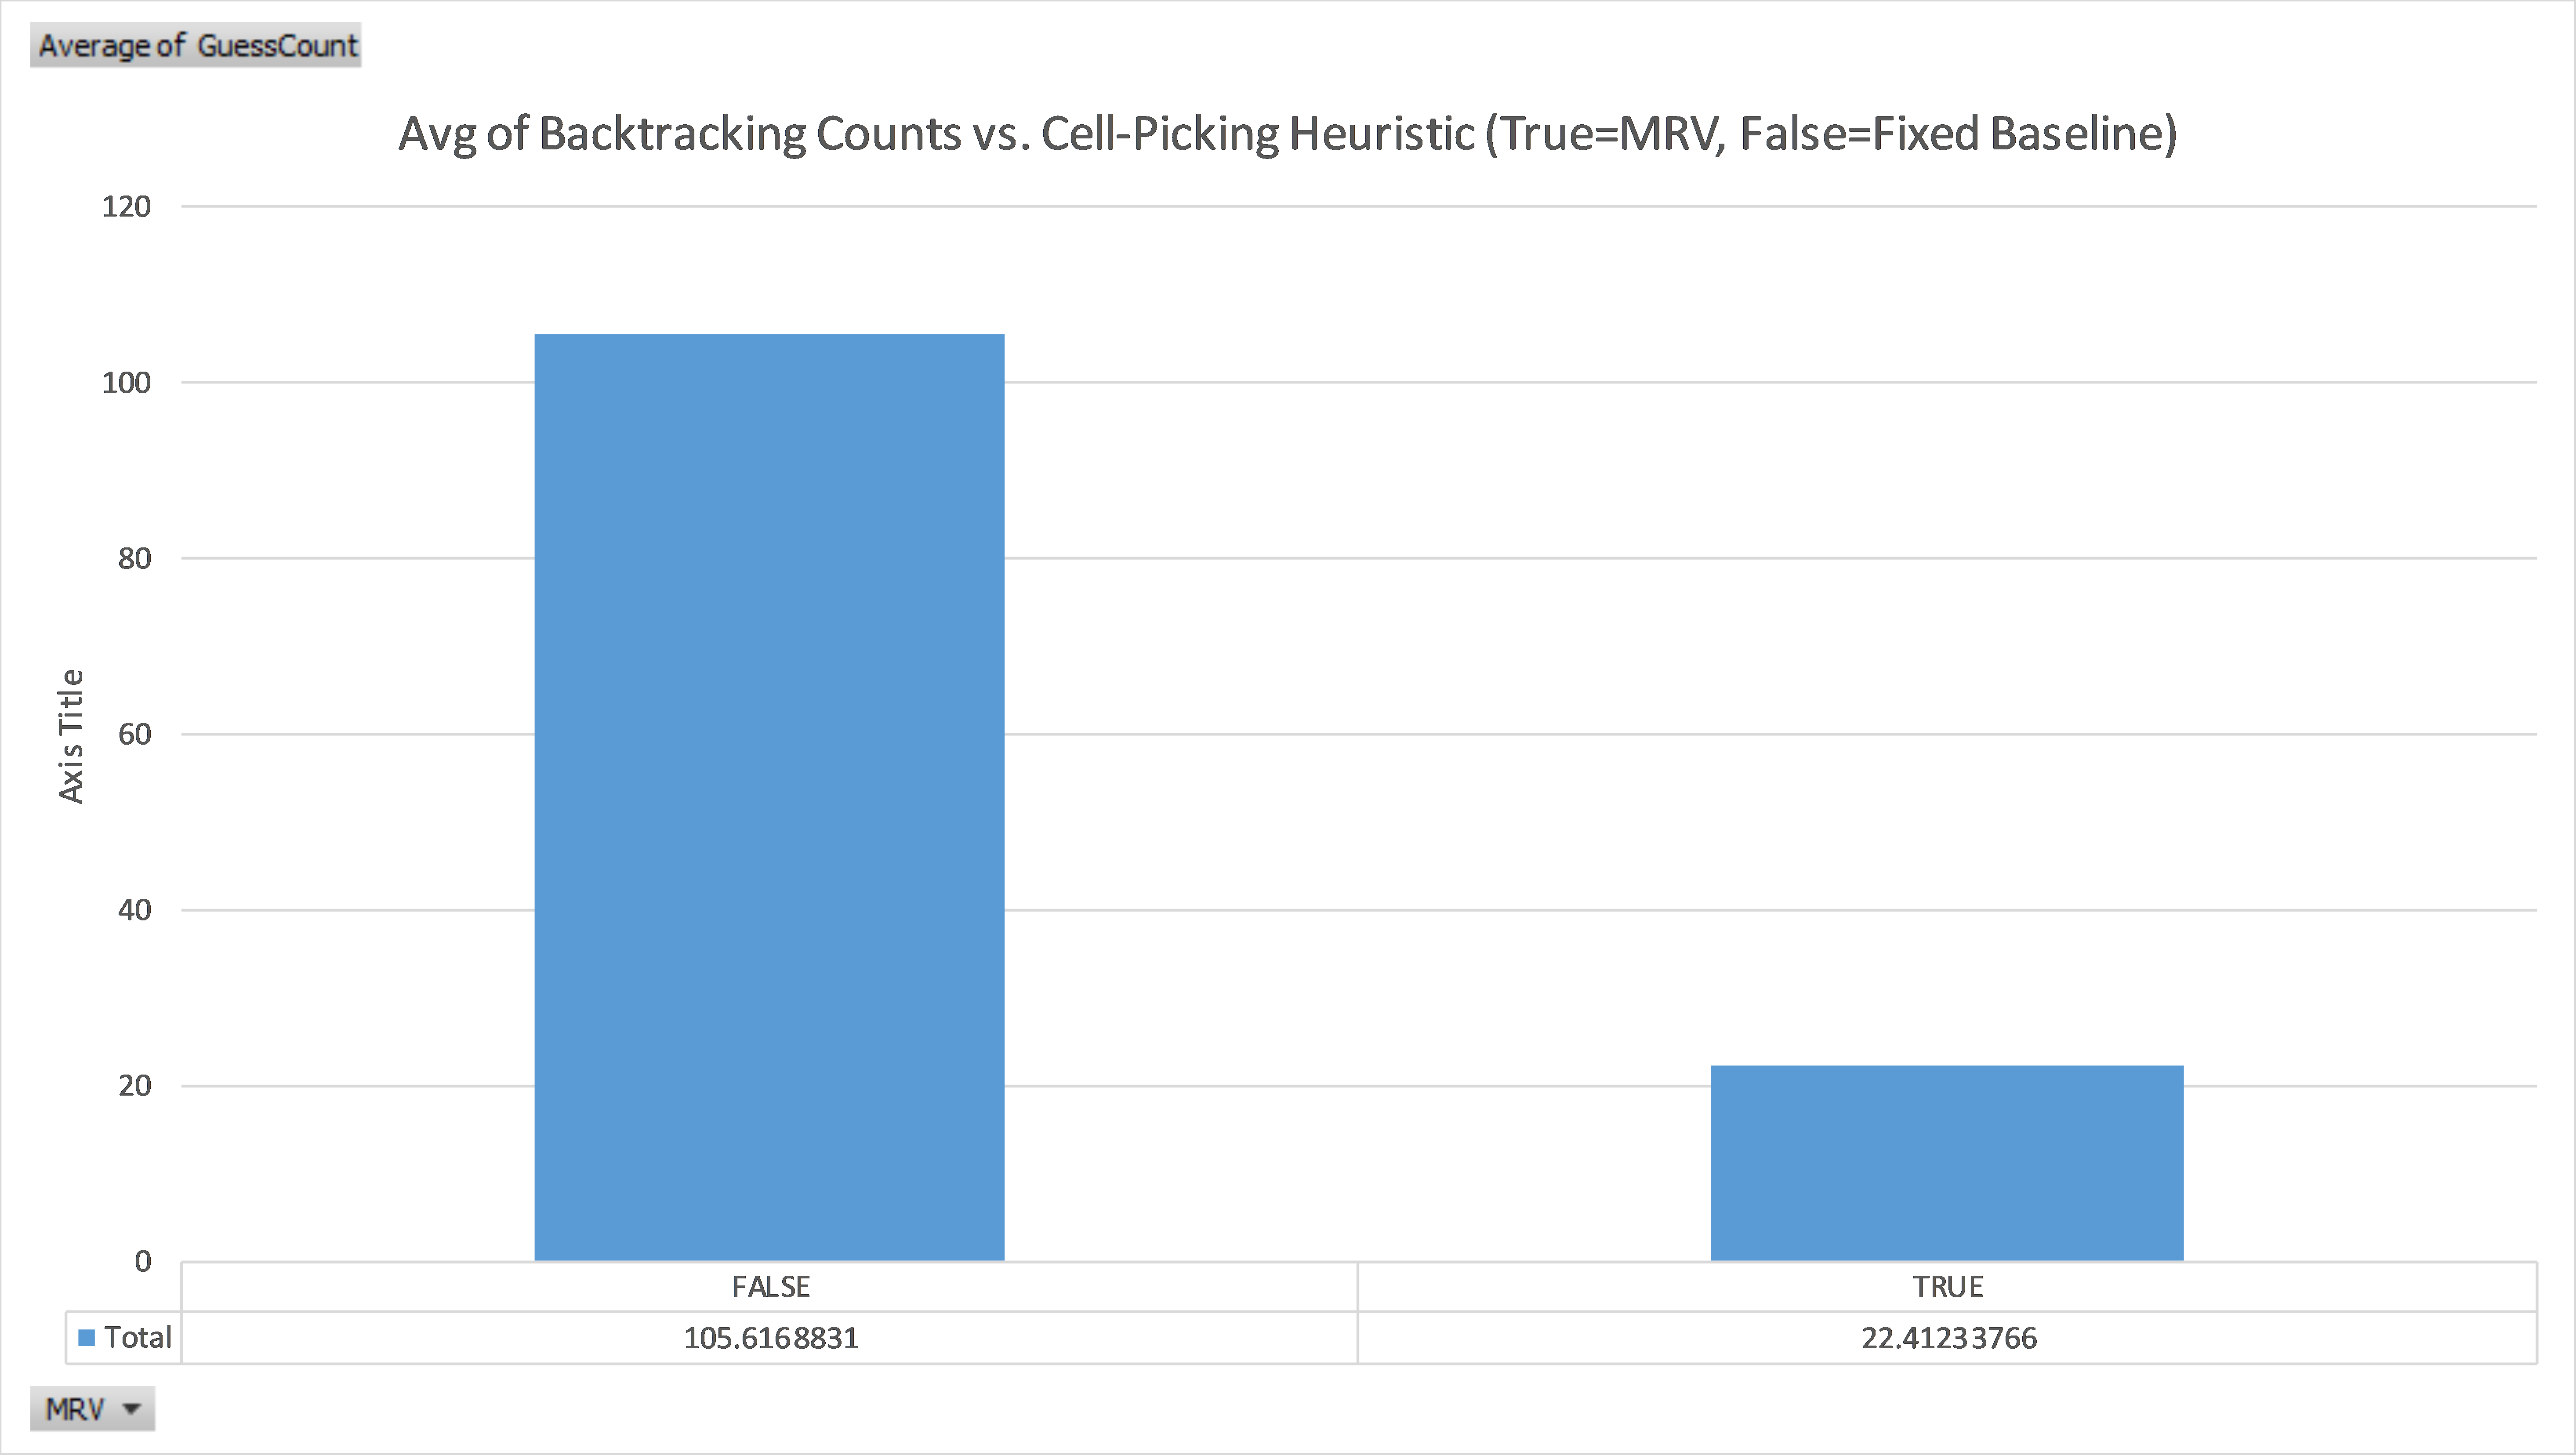
\includegraphics[scale=0.4]{plots/avg-backtrack-count-vs-cell-picking-heuristic.png}\\
	\end{tabular}
	\caption{Average Backtrack Count vs. Cell-Picking Heuristic}%
	\label{fig:avg_backtrack_count_vs_cell_heuristic}%
\end{figure}

Examining the backtracking behavior more deeply, we can see that there was generally more backtracking for the more difficult puzzles, as rated by the experts.  The total and average backtrack counts versus the expert puzzle difficulty can be seen in in figure \ref{fig:total_backtrack_vs_diff} and figure \ref{fig:avg_backtracks_vs_diff}, respectively.\\

\begin{figure}[H]%
	\centering\begin{tabular}{c}
		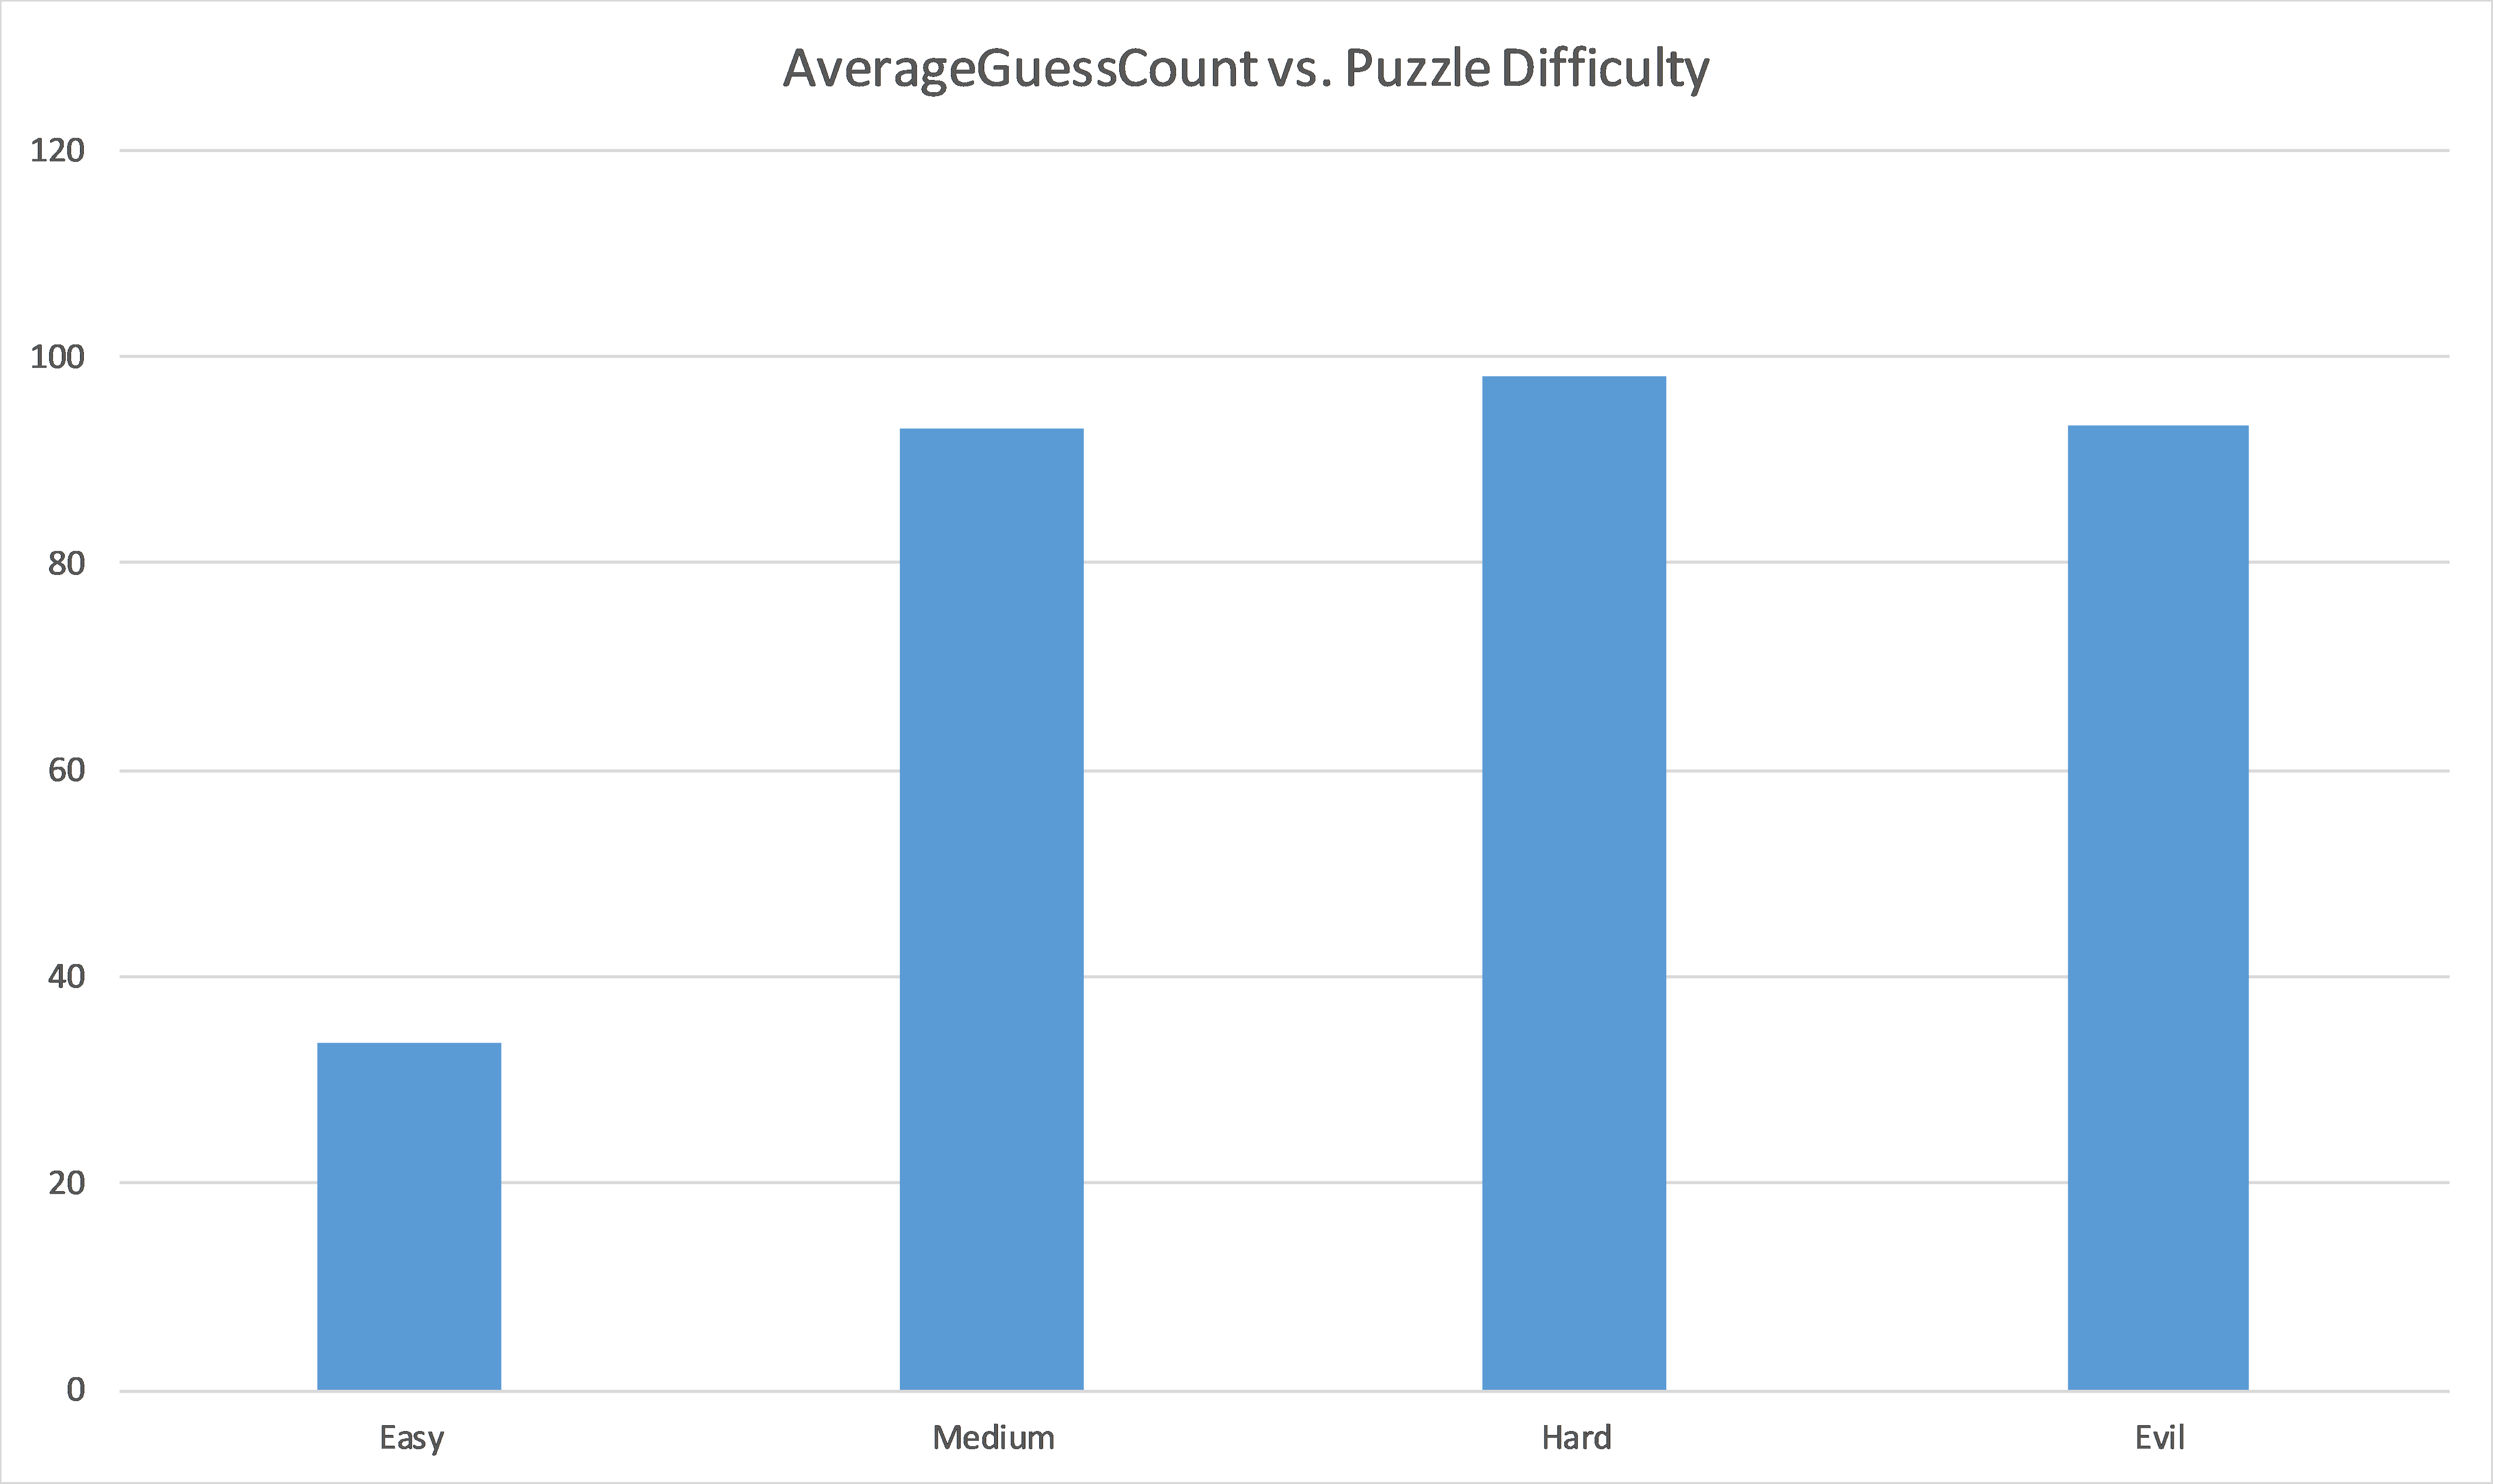
\includegraphics[scale=0.4]{plots/avg-guess-count-vs-puzzle-diff.png}\\
	\end{tabular}
	\caption{Average Backtracks/Guesses vs. Expert Puzzle Difficulty}%
	\label{fig:avg_backtracks_vs_diff}%
\end{figure}

\begin{figure}[H]%
	\centering\begin{tabular}{c}
		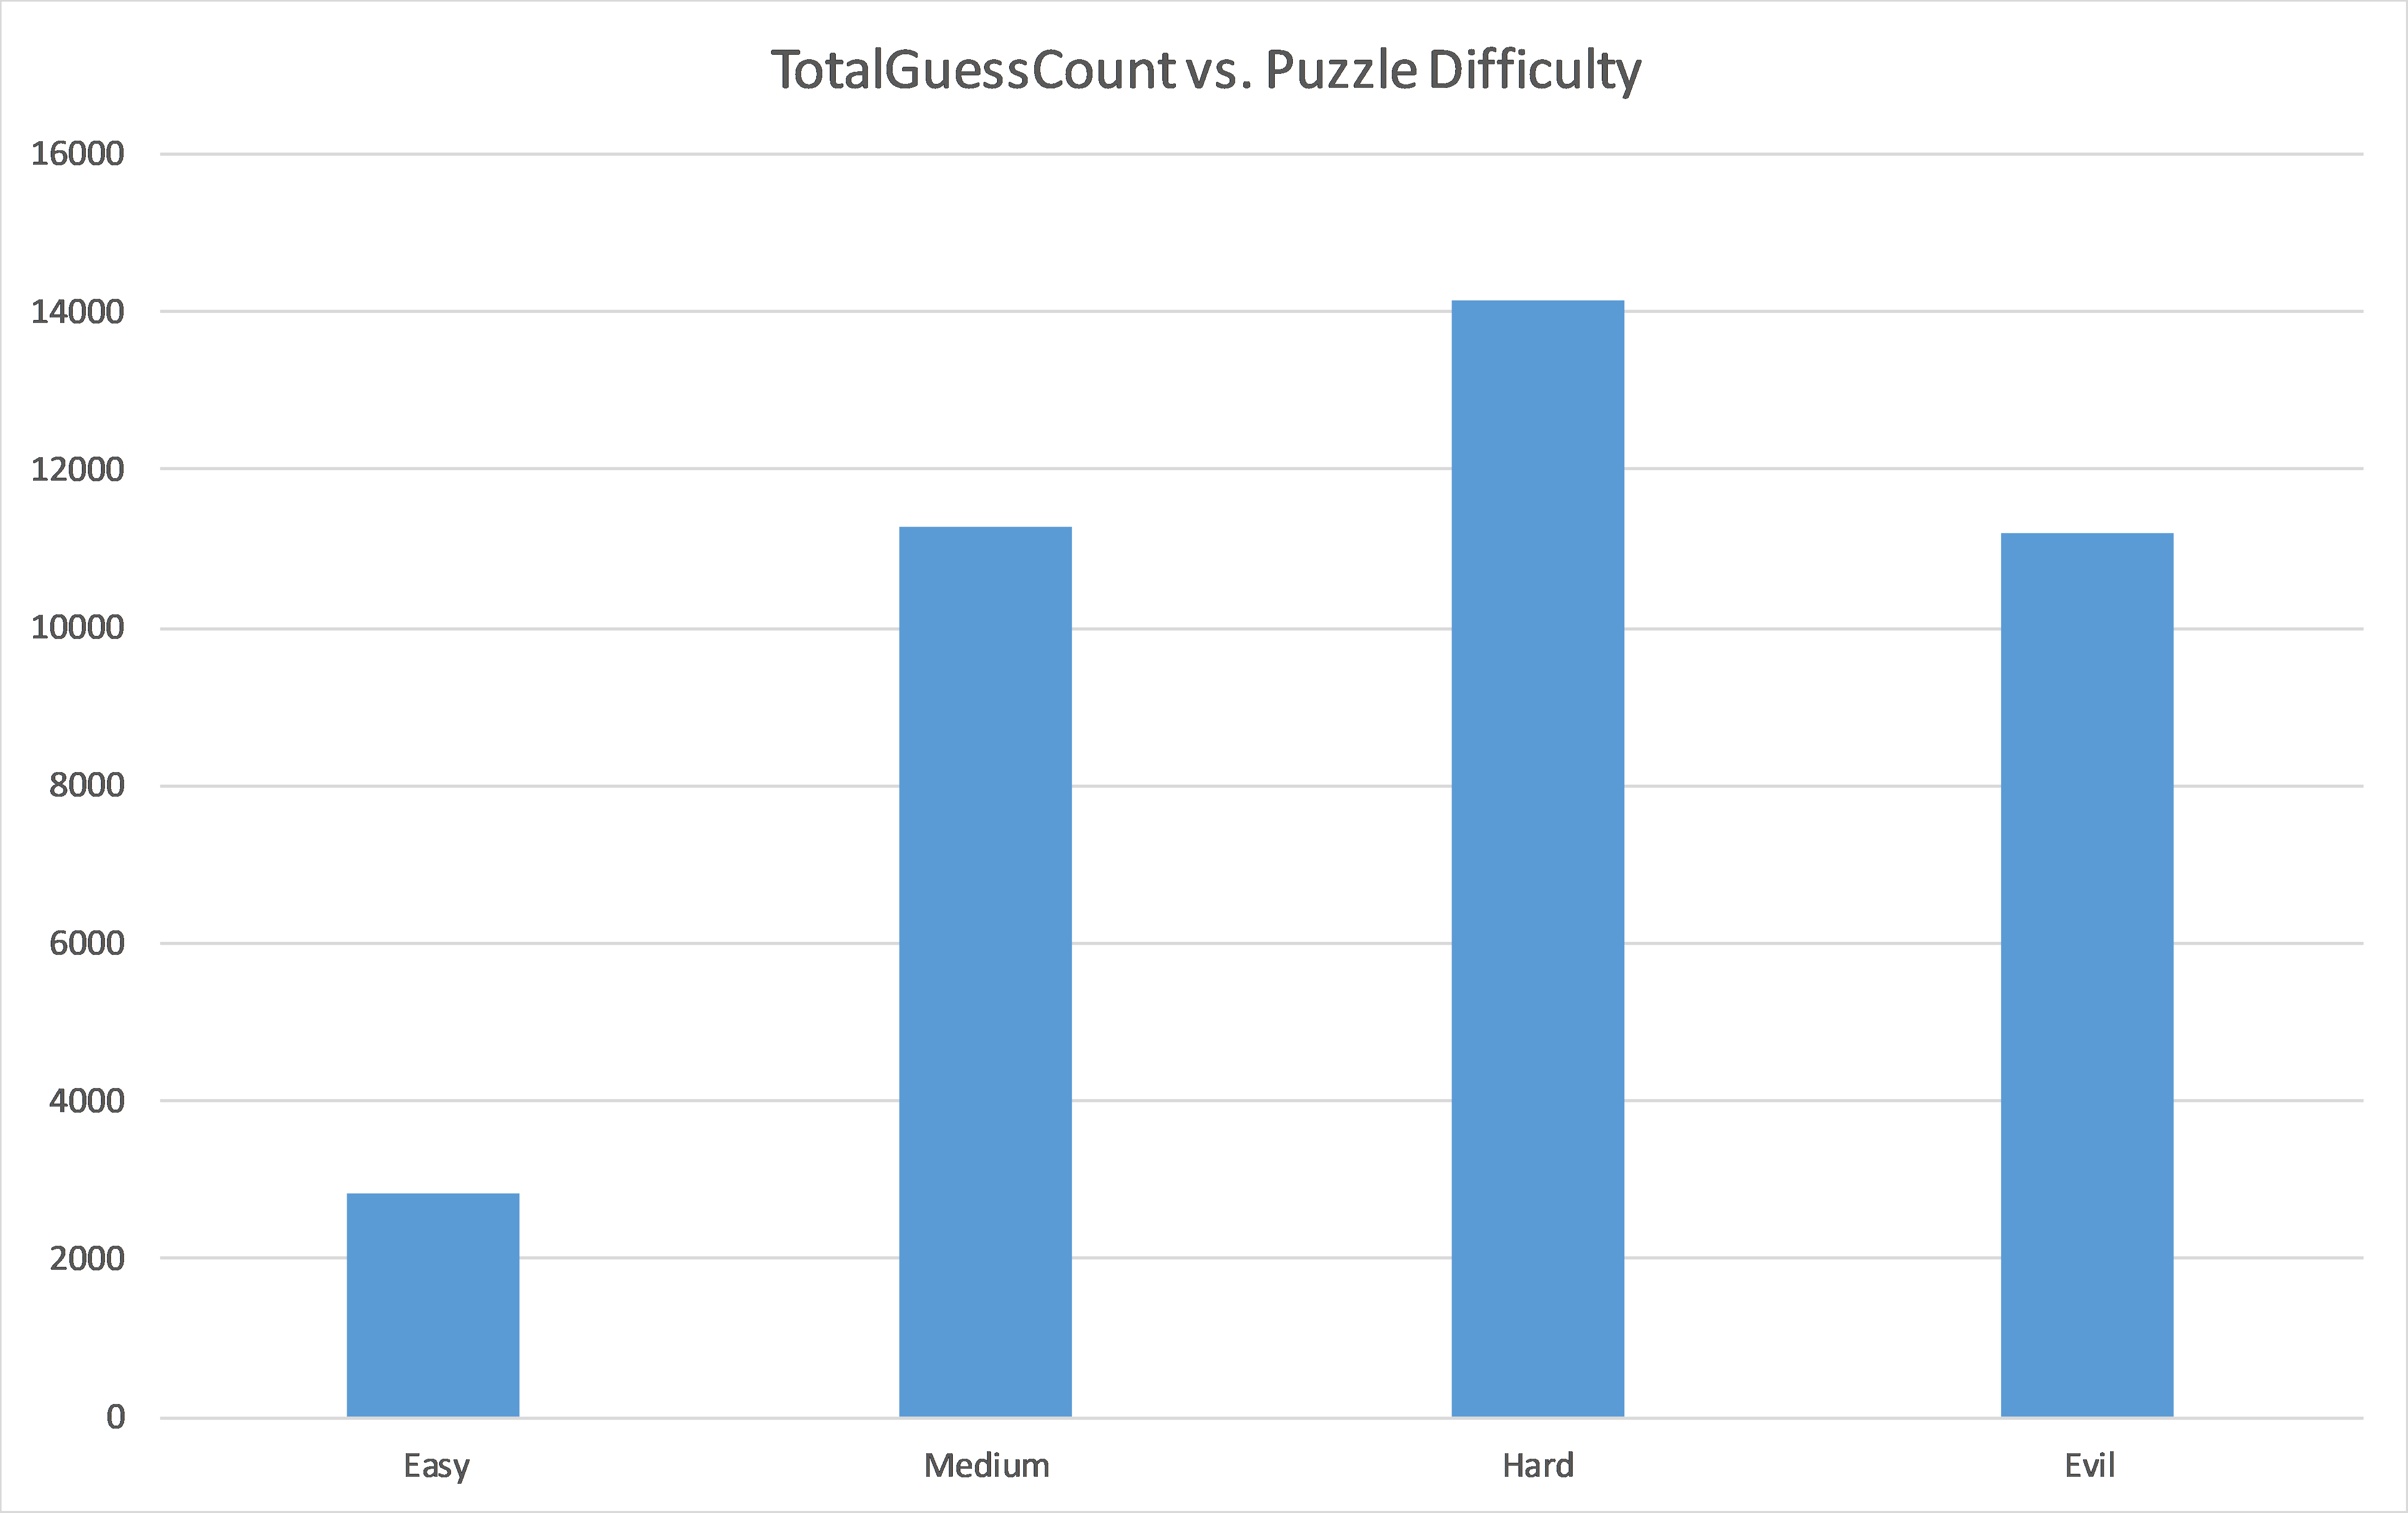
\includegraphics[scale=0.4]{plots/total-guess-count-vs-puzzle-diff.png}\\
	\end{tabular}
	\caption{Total Backtracks/Guesses vs. Expert Puzzle Difficulty}%
	\label{fig:total_backtrack_vs_diff}%
\end{figure}

The overall breakdown of the average backtracking activity can be seen in figure \ref{fig:avg_backtracks_vs_factors}. It is easy to see that the dominant factor affecting the backtracking across cell-picking method and single/pair/triple constraints was indeed the cell-picking method.\\

\begin{sidewaysfigure}
	\centering
	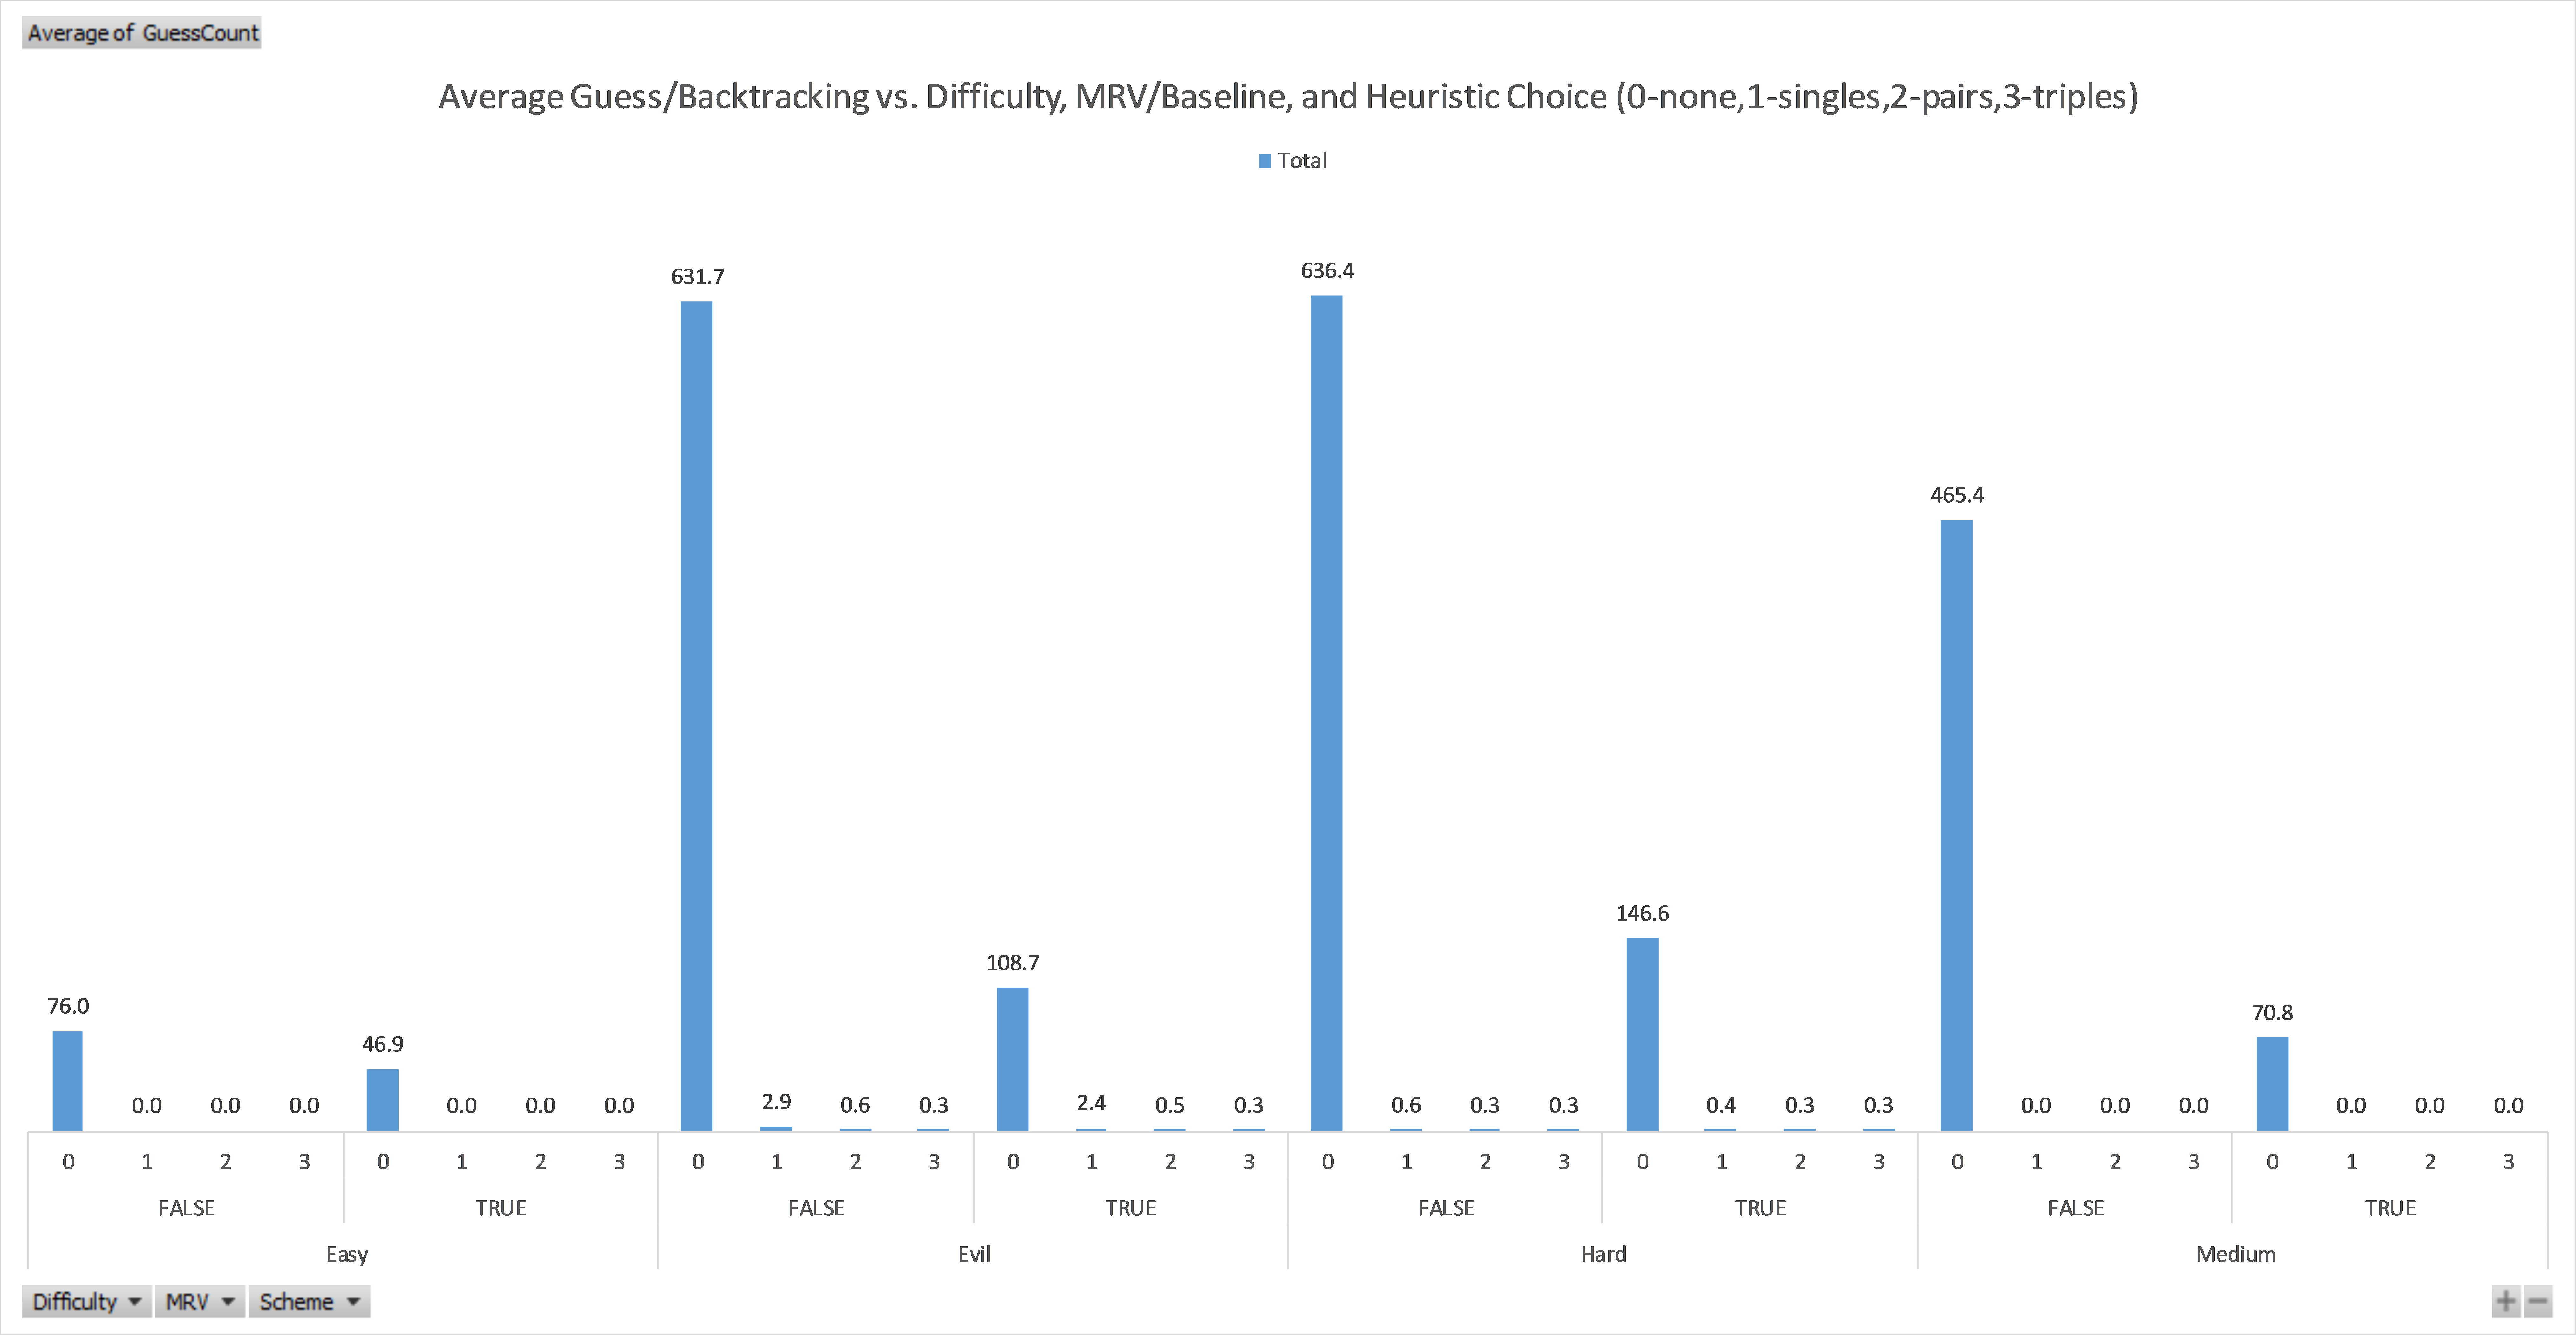
\includegraphics[scale=0.66]{plots/average-backtrack-guesses-vs-diff-scheme-heuristic.png}\\
	\caption{Average Backtracks/Guesses vs. Difficulty, Inference Scheme, Inference Heuristics}%
	\label{fig:avg_backtracks_vs_factors}%
\end{sidewaysfigure}

If we analyze the average number of cells filled in versus the expert puzzle difficulty (see figure \ref{fig:avg_filled_vs_diff}), we can see that the easy puzzles have more filled in cells. However, for medium, hard, and evil puzzles, there is not much of a difference.\\

\begin{figure}[H]%
	\centering\begin{tabular}{c}
		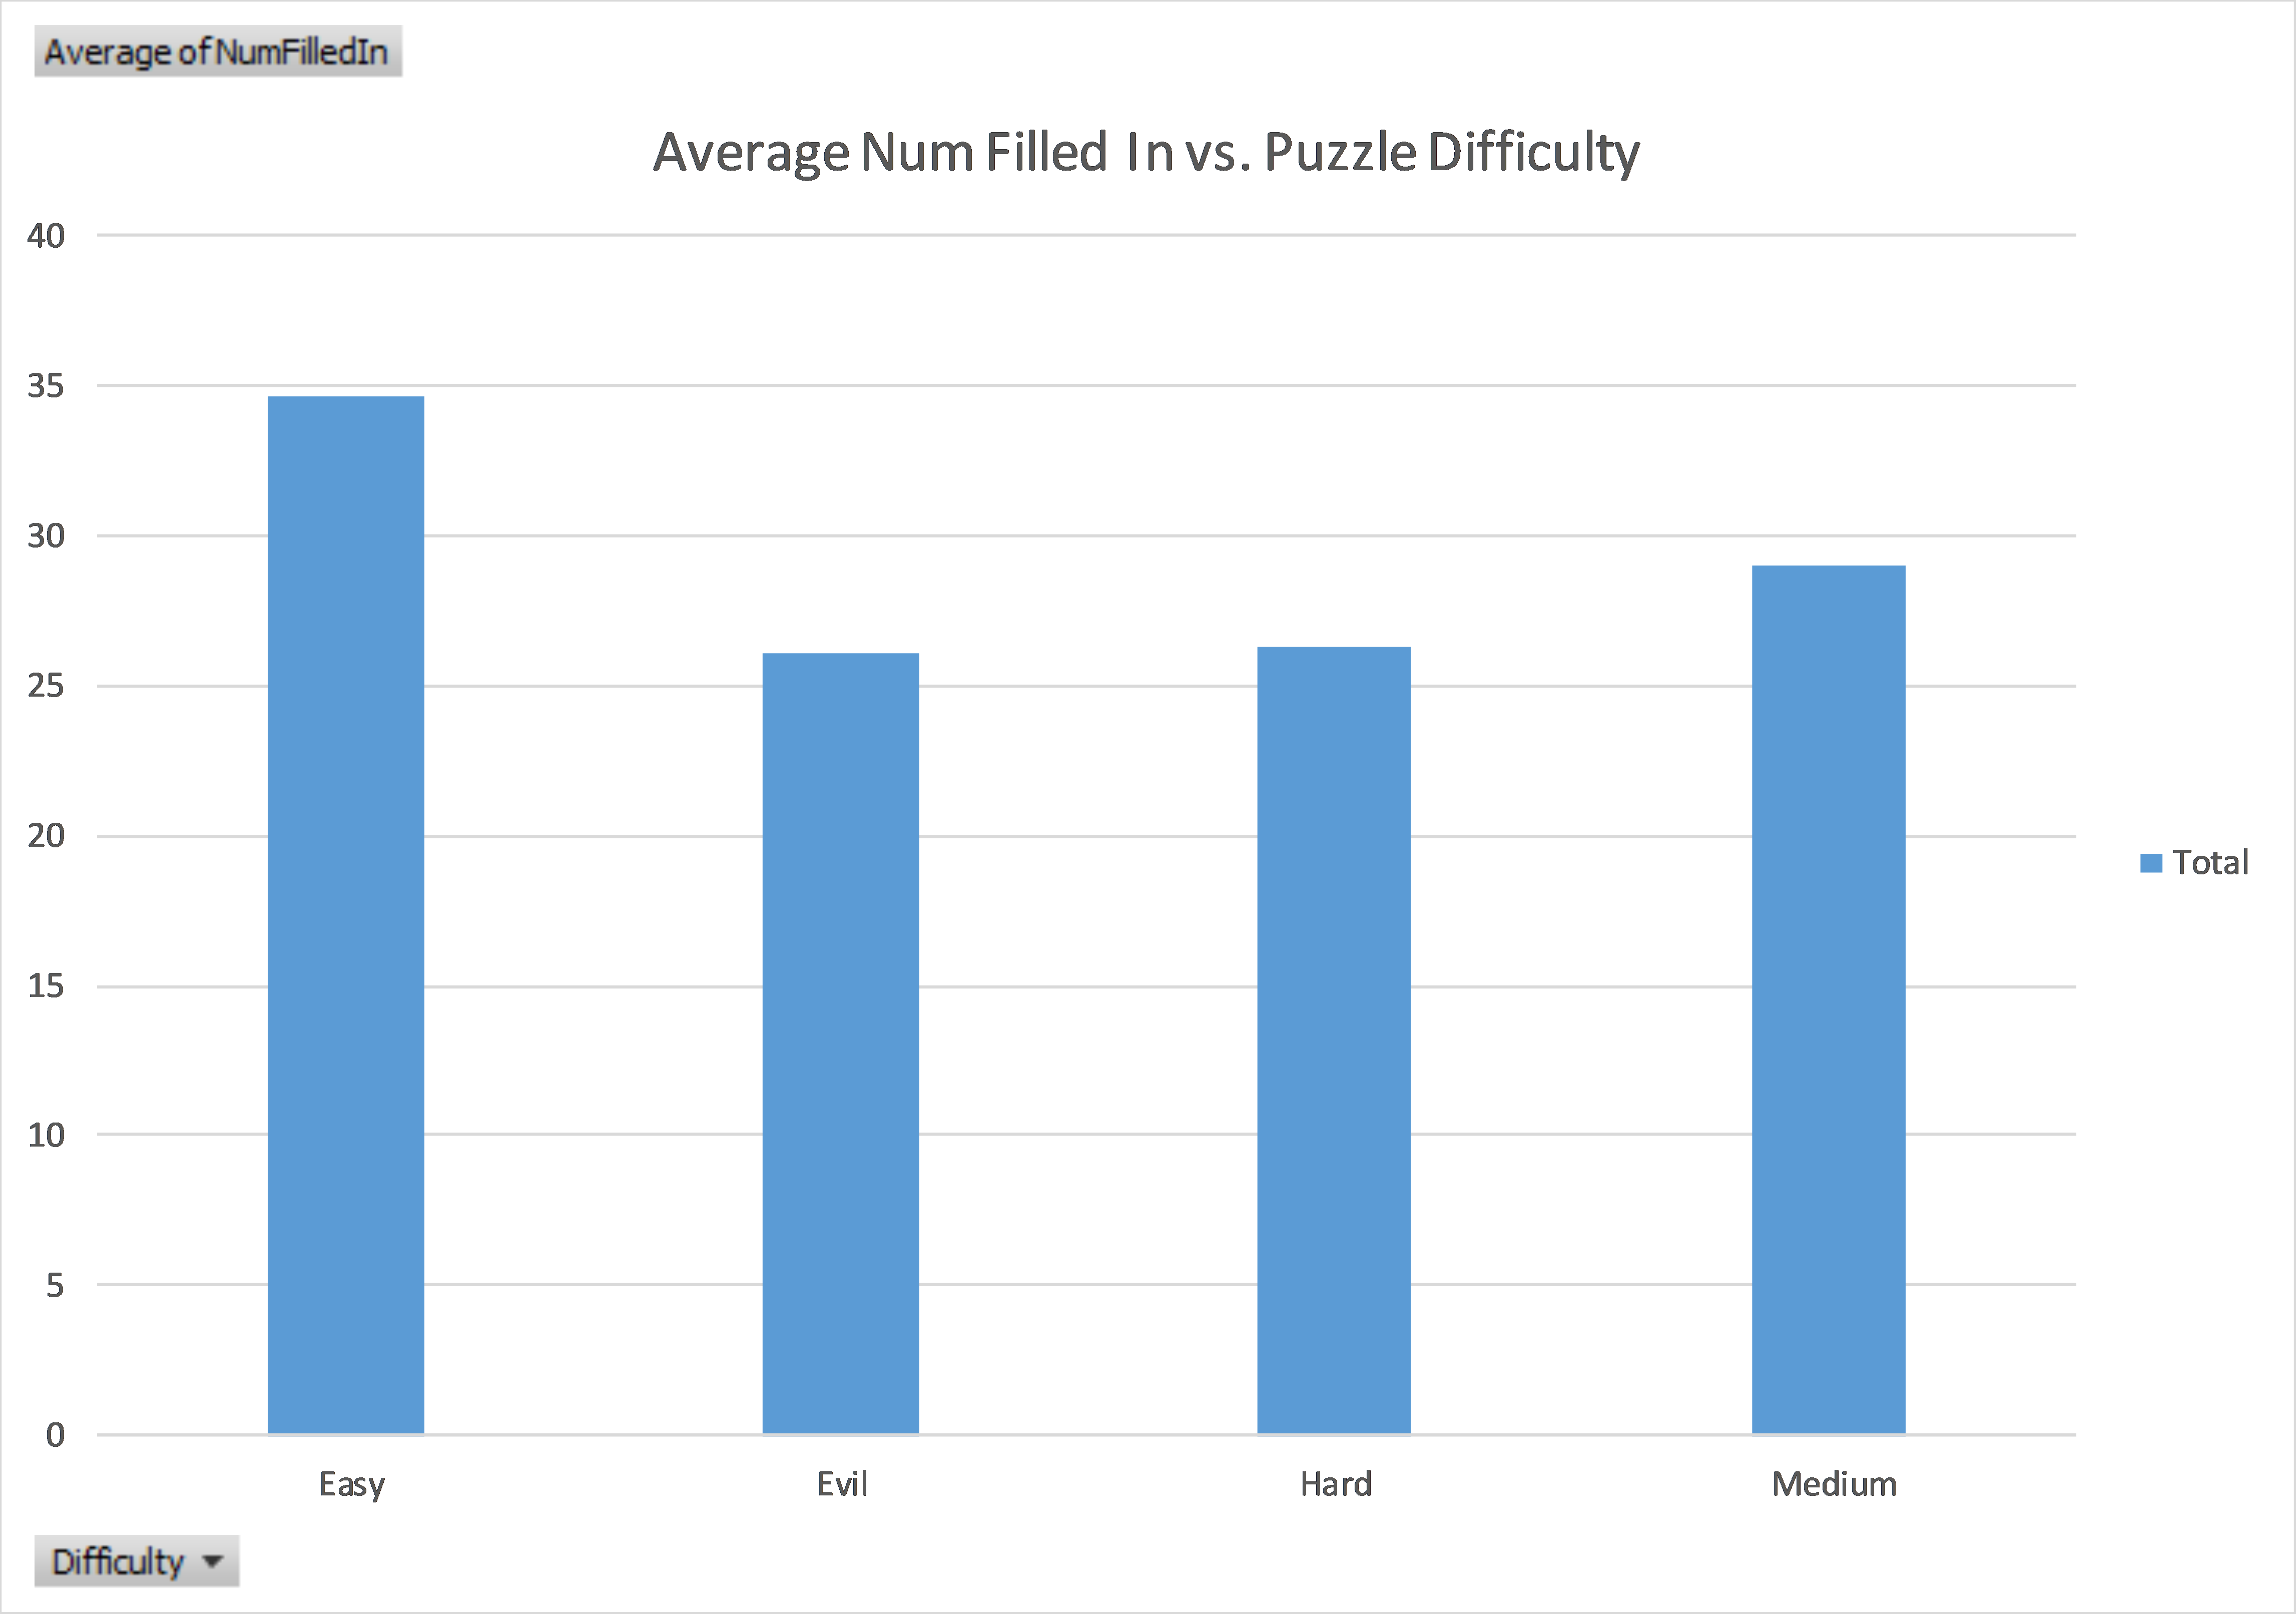
\includegraphics[scale=0.4]{plots/avg-num-filled-in-vs-puzzle-difficulty.png}\\
	\end{tabular}
	\caption{Average Number of Filled In Cells vs. Expert Puzzle Difficulty}%
	\label{fig:avg_filled_vs_diff}%
\end{figure}

\subsection{Distribution of Inference Constraints}
The distribution of the inference constraints (Naked Singles, Hidden Singles, Naked Pairs, Hidden Pairs, Naked Triples, Hidden Triples) across the expert puzzle difficulty ratings is mostly as we might expect. The easy puzzles show a reliance on Naked Singles, the medium puzzles show that we are using Hidden Singles in addition to the Naked Singles, the hard puzzles add Hidden Pairs to the mix, and finally, the evil puzzles show that we are now also utilizing Naked Pairs. We can also see that the evil puzzles occasionally utilize both the Hidden Triples and Naked Triples. The distribution is shown in figure \ref{fig:dist_inf_vs_puzzle_diff}.\\

\begin{figure}[H]%
	\centering\begin{tabular}{c}
		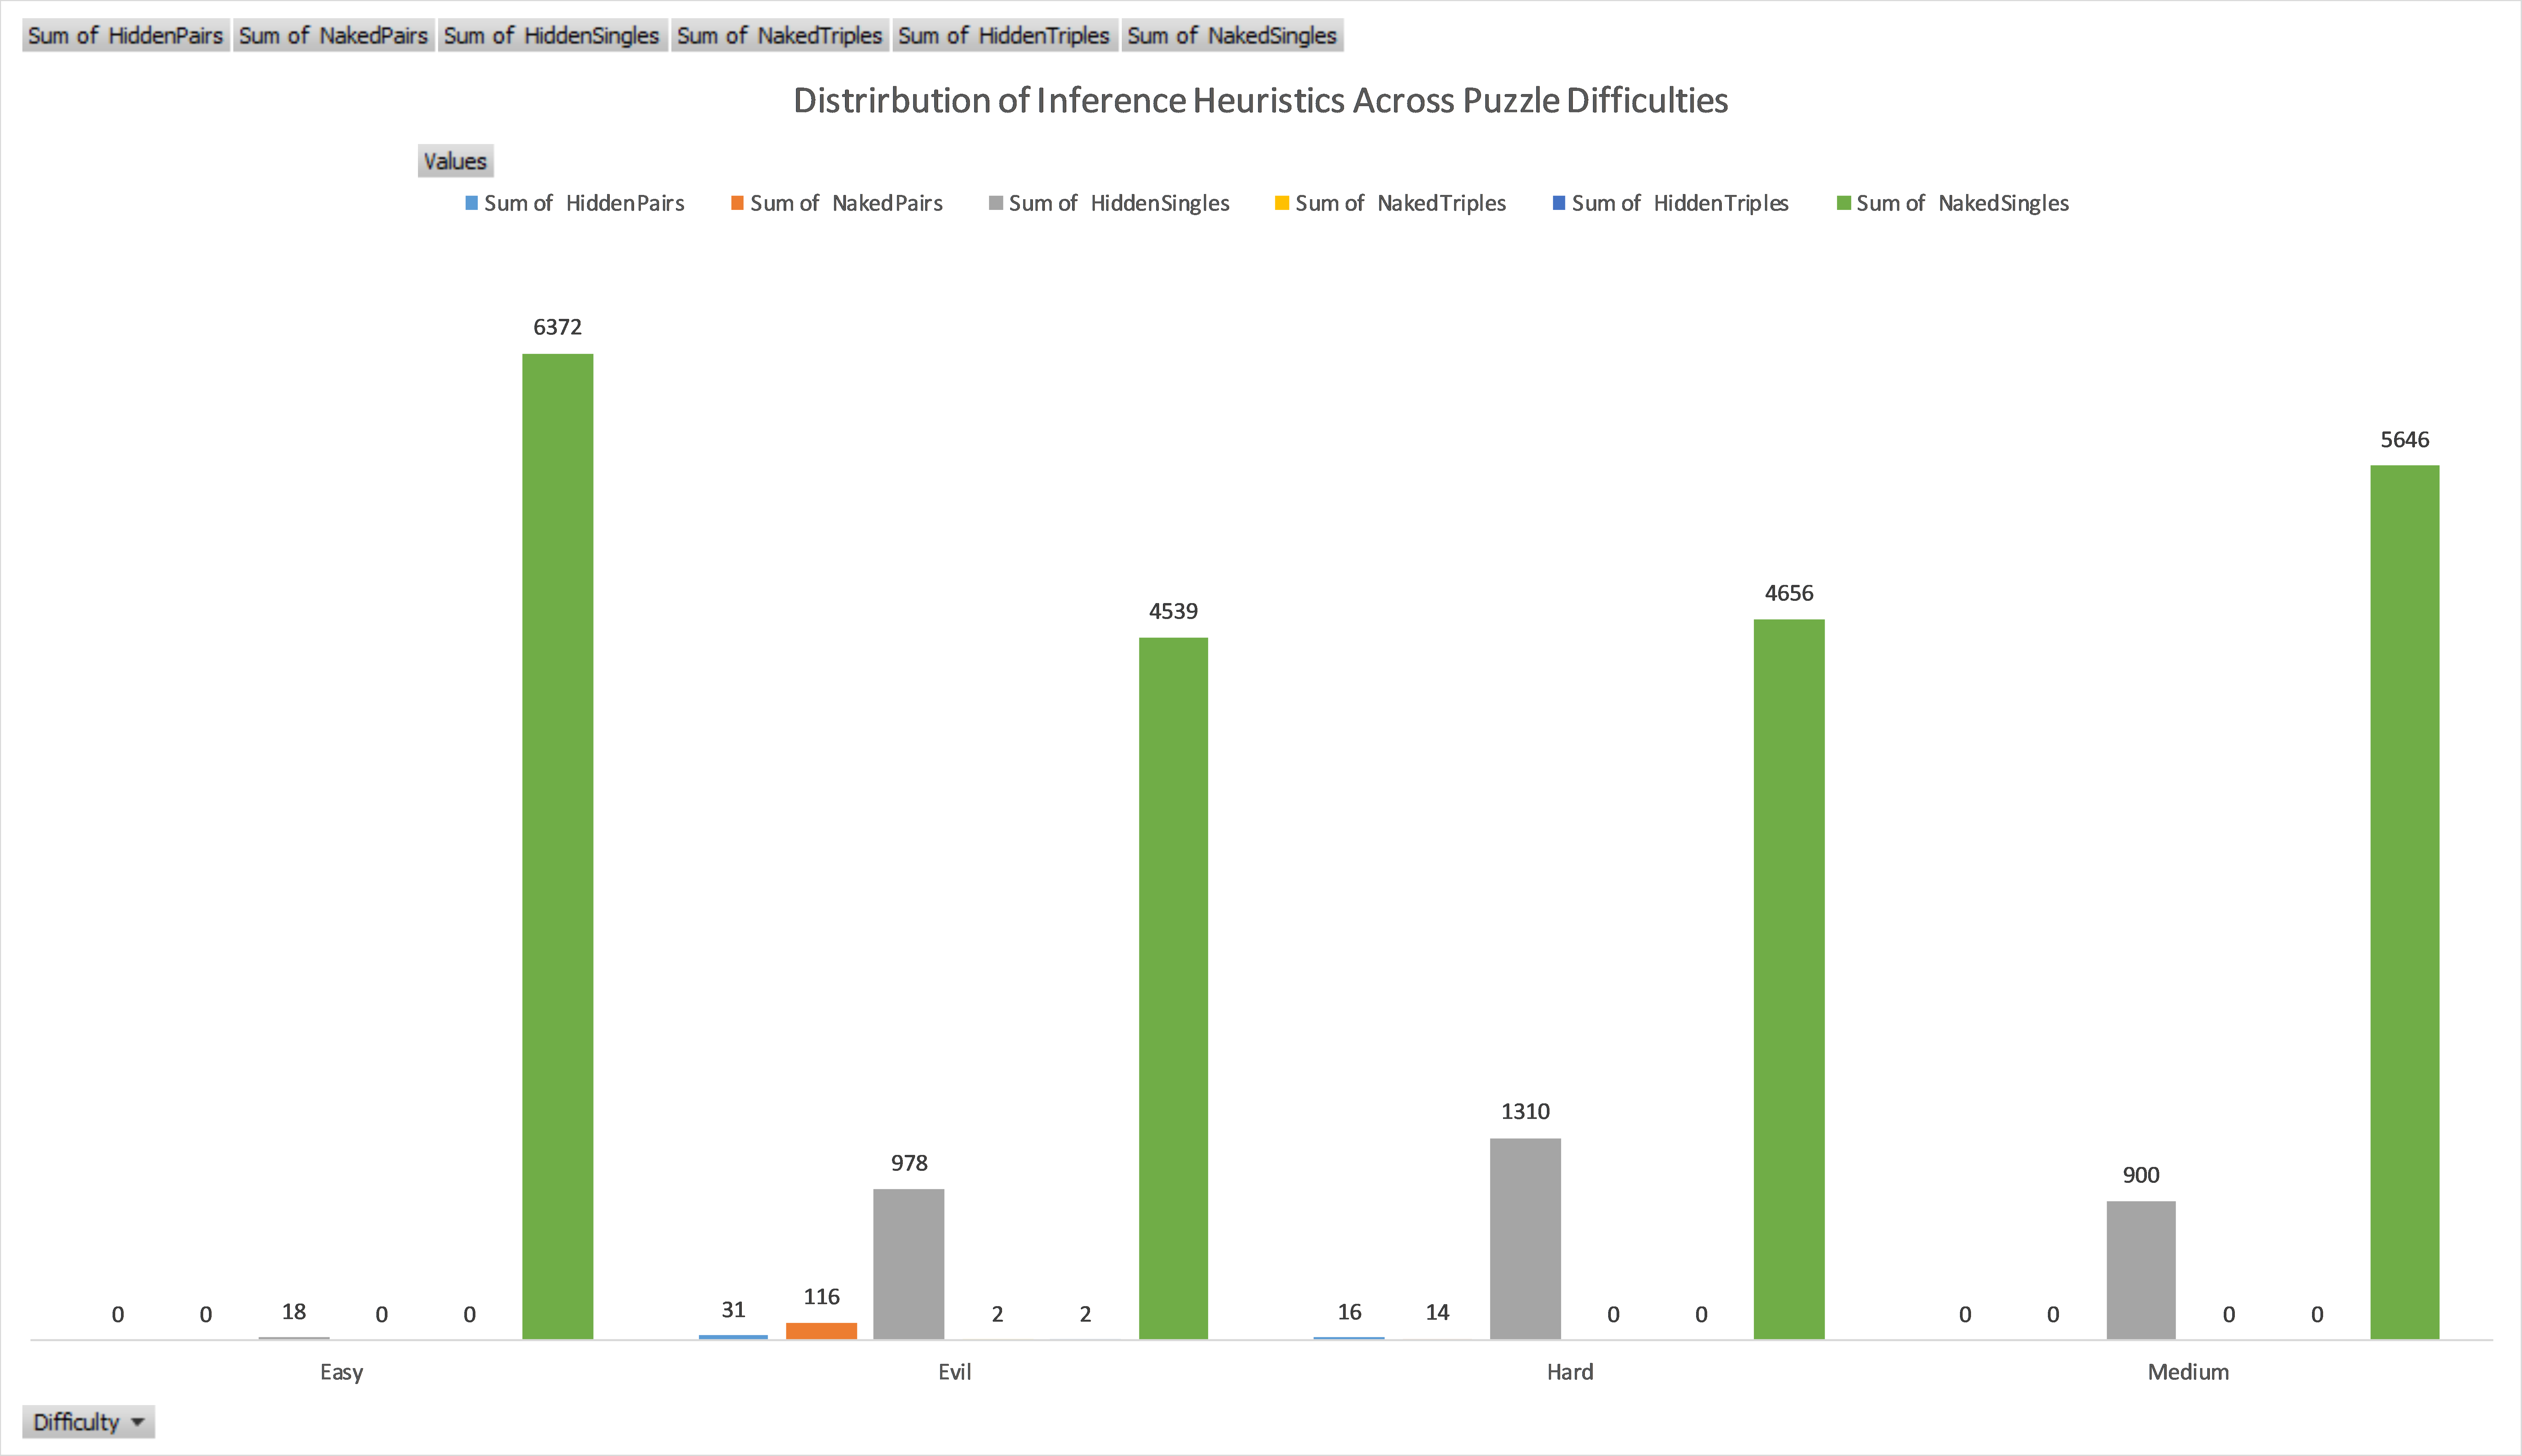
\includegraphics[scale=0.4]{plots/dist-inf-heuristics-vs-puzzle-diff.png}\\
	\end{tabular}
	\caption{Distribution of Inference Heuristics vs. Puzzle Difficulty}%
	\label{fig:dist_inf_vs_puzzle_diff}%
\end{figure}

Across the puzzles themselves, we see that there were only a few more difficult puzzles (numbers 4 and 26, and, to a lesser extent, number 60) that relied on more inference heuristics. We can also see that some puzzles only utilized one inference heuristic. Figure \ref{fig:dist_inf_vs_puzzle_num} shows the overall distribution over the individual puzzles.\\ 

\begin{sidewaysfigure}
	\centering
	\includegraphics[scale=0.50]{plots/dist-inf-heuristics-vs-puzzle-number.png}\\	
	\caption{{Distribution of Inference Heuristics vs. Puzzle Number}}
	\label{fig:dist_inf_vs_puzzle_num}%
\end{sidewaysfigure}

When we examine the distribution of total backtracking across the inference heuristics and take into account the cell-picking method, we can see that when we are using the baseline cell-picking method, we can see the increased backtracking activity, as discussed previously. What is more interesting is that for the single/pairs/triples, we see that the use of these heuristics in backtracking is relatively evenly distributed across the two cell-picking methods. The distribution can be seen in figure \ref{fig:total_backtracks_vs_mrv_heuristic}.

\begin{figure}[H]%
	\centering\begin{tabular}{c}
		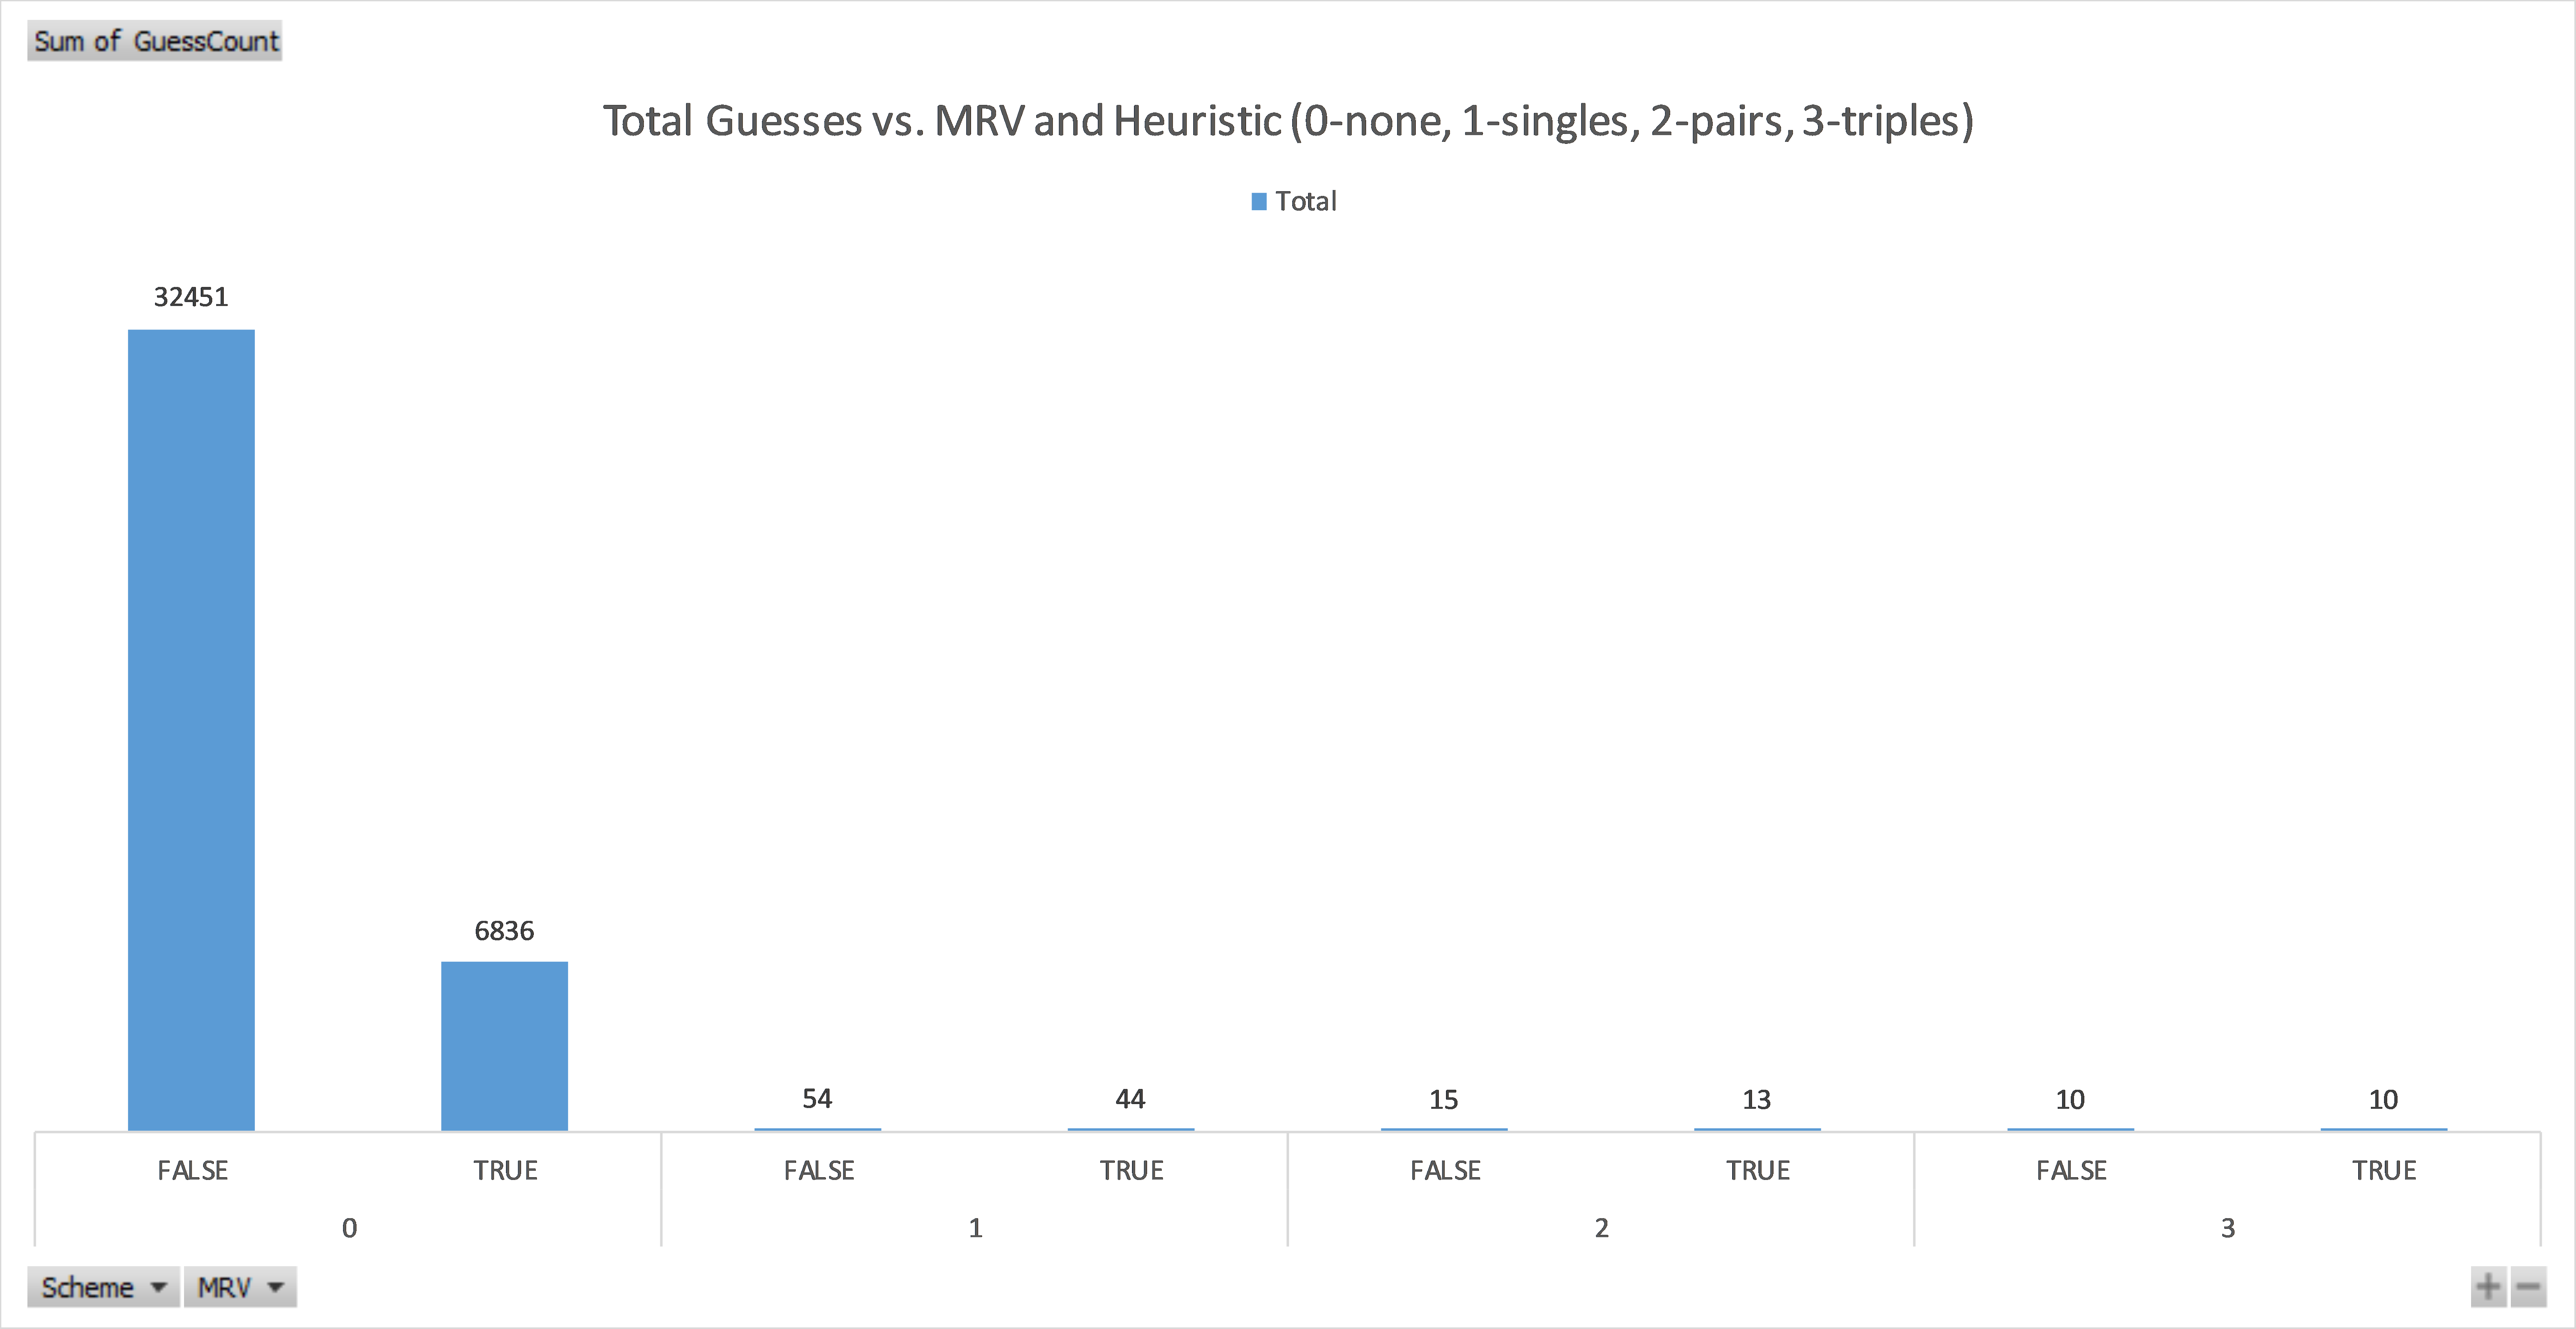
\includegraphics[scale=0.4]{plots/total-backtrack-guesses-vs-mrv-and-heuristic.png}\\
	\end{tabular}
	\caption{Total Backtracks/Guesses vs. MRV/Baseline and Heuristic}%
	\label{fig:total_backtracks_vs_mrv_heuristic}%
\end{figure}

\section{Discussion}
Across all of the experimental configurations, roughly 98\% of the puzzles were solved within 1000 steps. While not in the scope of this experimental effort, if the step limit had been increased, we are confident that all of the puzzles would have been solved. The total time taken for the 616 puzzles was less than 1 second, demonstrating the efficiency of the overall solution. Using the MRV method to pick the cell helped keep backtracking activity to a minimum and the inference of constraint heuristics was also effective, especially the simpler single constraints. With more difficult puzzles, we could see that the more complex pair/triple constraints were also utilized. We speculate that given a greater variety of test puzzles, especially more puzzles that would have been rated hard/evil by the experts, we would see even further use of the pair/triple constraints.\\
\\
Taking into consideration the approximately 1.1 millisecond per puzzle solving time and the not insubstantial total backtracking counts, we might surmise that future work should focus on how to cut down backtracking activity. The puzzle solving time is reasonable, especially considered as merely \enquote{wall time}, but there is likely room to improve on the backtracking. We might investigate more effective cell-picking methods and additional approaches for finding useful constraints. To assess the generality of our approach, we might test on both a much larger number of Sudoku puzzles as well as novel Sudoku configurations beyond the $9 \times 9$ grid and/or $3 \times 3$ blocks.

\section{Code}
\begin{lstlisting}
#include <iostream>
#include <iomanip>
#include <random>
#include <chrono>
#include <vector>
#include <string>
#include <set>
#include <algorithm>
#include <fstream>
#include <map>

using namespace std;

//#define SUDOKU_DEBUG

std::map<int, string> board_diff;

class Inferer {
    int board[9][9];
    int puzzle_no;
    bool MRV;
    int scheme;

    // Assignment and domain restriction transcripts
    vector<vector<pair<int, int>>>                       assignments;
    vector<vector<pair<pair<int, int>, int>>>            cell_restrict;
    vector<vector<pair<pair<int, int>, int>>>            row_restrict;
    vector<vector<pair<pair<int, int>, int>>>            col_restrict;
    vector<vector<pair<pair<int, int>, pair<int, int>>>> block_restrict;

    // Search and Inference Stats
    int guess_count        = 0;
    int naked_single_apps  = 0;
    int hidden_single_apps = 0;
    int naked_pair_apps    = 0;
    int hidden_pair_apps   = 0;
    int naked_triple_apps  = 0;
    int hidden_triple_apps = 0;

    // With at most 9 elements in each set, the asymptotic time complexity advantage
    // of unordered_set vs. set is irrelevant. We can experiment with both to see
    // which has better time and space performance.

    // Possible values by cell: if assigned, set will be emtpy
    vector<vector<set<int>>> cell;

    // Possibly locations for values by row, column, and block: if assigned, set will be empty
    vector<vector<set<int>>> row;              // row[row #][value]:     set of col #'s
    vector<vector<set<int>>> col;              // col[col #][value]:     set of row #'s
    vector<vector<set<pair<int,int>>>> block;  // block[block #][value]: set of coords


    void increment(pair<int, int> &p, int j_low, int j_high) {
        ++p.second;
        if (p.second >= j_high) {
            p.second = j_low;
            ++p.first;
        }
    }

public:
    Inferer(int **b, int p_no, bool mrv, int s) : puzzle_no(p_no), MRV(mrv), scheme(s) {
        new_layer();
        for (int i = 0; i < 9; ++i)
            for (int j = 0; j < 9; ++j)
                board[i][j] = b[i][j];
        initialize();
    }

    int get_guess_count() { return guess_count; }

    void print() {
        int filled = 0;
        for (int i = 0; i < 9; ++i)
            for (int j = 0; j < 9; ++j)
                if (board[i][j] > 0)
                    ++filled;
        #ifdef SUDOKU_DEBUG
            cout << endl;
            for (int i = 0; i < 9; ++i) {
                for (int j = 0; j < 9; ++j)
                    cout << ' ' << board[i][j];
                cout << endl;
            }
            cout << endl;
            cout << "Puzzle #: " << puzzle_no << endl;
            cout << "MRV? " << boolalpha << MRV << endl;
            cout << "Scheme: " << scheme << endl;
            cout << "Completion: " << fixed << setprecision(1) << (100 * filled) / 81.0 << '%' << endl;;
            cout << "Guess count: " << guess_count << endl;
            cout << "Naked single applications:  " << naked_single_apps << endl;
            cout << "Hidden single applications: " << hidden_single_apps << endl;
            cout << "Naked pair applications:    " << naked_pair_apps << endl;
            cout << "Hidden pair applications:   " << hidden_pair_apps << endl;
            cout << "Naked triple applications:  " << naked_triple_apps << endl;
            cout << "Hidden triple applications: " << hidden_triple_apps << endl;
            cout << endl;
        #else
            cout << puzzle_no << ',' << board_diff[puzzle_no] << ","  << guess_count << ','
                 << boolalpha << MRV << ',' << scheme << ','
                 << fixed << setprecision(1) << 100 * filled / 81.0 << ','
                 << naked_single_apps << ',' << hidden_single_apps << ','
                 << naked_pair_apps << ',' << hidden_pair_apps << ','
                 << naked_triple_apps << ',' << hidden_triple_apps << endl;
        #endif
    }

    void new_layer() {
        assignments.emplace_back();
        cell_restrict.emplace_back();
        row_restrict.emplace_back();
        col_restrict.emplace_back();
        block_restrict.emplace_back();
    }

    int infer() {
        switch(scheme) {
            case 3:  return up_to_triples();
            case 2:  return up_to_pairs();
            case 1:  return up_to_singles();
            default: return no_inference();
        }
    }

    set<int> get_guess_domain(pair<int, int> &p) {
        if (MRV) {
            int min_size = 10;
            for (int i = 0; i < 9; ++i)
                for (int j = 0; j < 9; ++j) {
                    int d_size = cell[i][j].size();
                    if (0 < d_size && d_size < min_size) {
                        p.first = i;
                        p.second = j;
                        min_size = d_size;
                    }
                }
            return cell[p.first][p.second];
        }
        else {
            for (int i = 0; i < 9; ++i)
                for (int j = 0; j < 9; ++j)
                    if (board[i][j] == 0) {
                        p.first = i;
                        p.second = j;
                        return cell[i][j];
                    }
        }
        return set<int>();
    }

    bool complete() {
        for (int i = 0; i < 9; ++i)
            for (int j = 0; j < 9; ++j)
                if (board[i][j] == 0) return false;
        return true;
    }
    
    bool verify() {
        return initialize();
    }

    int guess(pair<int, int> &var, int val) {
        #ifdef SUDOKU_DEBUG
            cout << "Guess " << val << " for (" << var.first << ", " << var.second << ")" << endl;
        #endif
        ++guess_count;
        return assign(var.first, var.second, val);
    }

    // Initializes variable domains for inference. Can also be used to perform
    // verification on a completed puzzle.
    bool initialize() {
        reset();
        for (int i = 0; i < 9; ++i) {
            for (int j = 0; j < 9; ++j) {
                int v = board[i][j];
                if (v > 0) {
                    if (assign(i, j, v, false) == 2) return false;
                }
            }
        }
        return true;
    }

    void reset() {
        cell  = vector<vector<set<int>>>(9, vector<set<int>>(9, set<int>({ 1 ,2, 3, 4, 5, 6, 7, 8, 9 })));
        row   = vector<vector<set<int>>>(9, vector<set<int>>(9, set<int>({ 0, 1 ,2, 3, 4, 5, 6, 7, 8 })));
        col   = vector<vector<set<int>>>(9, vector<set<int>>(9, set<int>({ 0, 1 ,2, 3, 4, 5, 6, 7, 8 })));
        block = vector<vector<set<pair<int,int>>>>(9, vector<set<pair<int, int>>>(9, set<pair<int, int>>()));
        for (int i = 0; i < 9; ++i)
            for (int j = 0; j < 9; ++j) {
                pair<int, int> p(i, j);
                int b = get_block(p);
                for (int k = 0; k < 9; ++k)
                    block[b][k].insert(p);
            }
    }

    int get_block(const pair<int, int> &p) {
        return 3 * (p.first / 3) + (p.second / 3);
    }

    /***********************
     * Variable Assignment *
     ***********************/
     // Return values:
     //   1 - successful assignment
     //   2 - conflict (i.e. empty domain for unassigned variable), need to backtrack
    int assign(int i, int j, int v, bool remember = true) {
        // Check whether assignment is valid
        if (cell[i][j].find(v) == cell[i][j].end())
            return 2;

        pair<int, int> p(i, j);
        int b = get_block(p);

        // Make assignment on board (if not during initialization)
        if (remember) {
            board[i][j] = v;
            assignments.back().push_back(p);
        }

        // Clear the sets to indicate assignment
        // (and prevent domain restriction from
        // returning empty domain error)
        clear_cell(i, j);
        clear_row(i, v);
        clear_col(j, v);
        clear_block(b, v);

        // Remove value from rest of row and column.
        // Remove coordinates from all other values.
        for (int k = 0; k < 9; ++k) {
            if (eliminate(i, k, v)) return 2;
            if (eliminate(k, j, v)) return 2;
            if (eliminate(i, j, k + 1)) return 2;
        }

        // Remove value from rest of block
        int bi = 3 * (i / 3);
        int bj = 3 * (j / 3);
        for (int x = bi; x < bi + 3; ++x)
            for (int y = bj; y < bj + 3; ++y)
                if(eliminate(x, y, v)) return 2;

        return 1;
    }

    // Reverse all assignments and domain restrictions made during inference
    // and from last guess, if any.
    void backtrack() {
        for (const pair<int, int> &p : assignments.back())
            board[p.first][p.second] = 0;
        assignments.pop_back();
        for (const pair<pair<int, int>, int> &p : cell_restrict.back())
            cell[p.first.first][p.first.second].insert(p.second);
        cell_restrict.pop_back();
        for (const pair<pair<int, int>, int> &p : row_restrict.back())
            row[p.first.first][p.first.second].insert(p.second);
        row_restrict.pop_back();
        for (const pair<pair<int, int>, int> &p : col_restrict.back())
            col[p.first.first][p.first.second].insert(p.second);
        col_restrict.pop_back();
        for (const pair<pair<int, int>, pair<int, int>> &p : block_restrict.back())
            block[p.first.first][p.first.second].insert(p.second);
        block_restrict.pop_back();
    }

    /**********************
     * Domain restriction *
     **********************/
     // Return: true if restriction makes a domain empty,
     //         false otherwise
    bool eliminate(int i, int j, int v) {
        if (cell[i][j].erase(v)) {
            cell_restrict.back().emplace_back(make_pair(i, j), v);
            if (cell[i][j].empty()) return true;
        }
        if (row[i][v - 1].erase(j)) {
            row_restrict.back().emplace_back(make_pair(i, v - 1), j);
            if (row[i][v - 1].empty()) return true;
        }
        if (col[j][v - 1].erase(i)) {
            col_restrict.back().emplace_back(make_pair(j, v - 1), i);
            if (col[j][v - 1].empty()) return true;
        }
        pair<int, int> p(i, j);
        int b = get_block(p);
        if (block[b][v - 1].erase(p)) {
            block_restrict.back().emplace_back(make_pair(b, v - 1), p);
            if (block[b][v - 1].empty()) return true;
        }
        return false;
    }

    // The following functions remember all elements in the set
    // before clearing it.
    void clear_cell(int i, int j) {
        for (int v : cell[i][j])
            cell_restrict.back().emplace_back(make_pair(i, j), v);
        cell[i][j].clear();
    }

    void clear_row(int i, int v) {
        for (int j : row[i][v - 1])
            row_restrict.back().emplace_back(make_pair(i, v - 1), j);
        row[i][v - 1].clear();
    }

    void clear_col(int j, int v) {
        for (int i : col[j][v - 1])
            col_restrict.back().emplace_back(make_pair(j, v - 1), i);
        col[j][v - 1].clear();
    }

    void clear_block(int b, int v) {
        for (const pair<int, int> &p : block[b][v - 1])
            block_restrict.back().emplace_back(make_pair(b, v - 1), p);
        block[b][v - 1].clear();
    }

    /*******************
     * Inference Rules *
     *******************/
     // Return values:
     //   0 - no application found
     //   1 - application found and applied
     //   2 - conflict, need to backtrack

    int naked_single() {
        for (int i = 0; i < 9; ++i)
            for (int j = 0; j < 9; ++j)
                if (cell[i][j].size() == 1) {
                    #ifdef SUDOKU_DEBUG
                        cout << "Naked single found in cell (" << i << ", " << j << ')' << endl;
                    #endif
                    ++naked_single_apps;
                    return assign(i, j, *cell[i][j].begin());
                }
        return 0;
    }

    int hidden_single() {
        for (int x = 0; x < 9; ++x) {
            for (int v = 0; v < 9; ++v) {
                if (row[x][v].size() == 1) {
                    #ifdef SUDOKU_DEBUG
                        cout << "Hidden single found in cell (" << x << ", " << *row[x][v].begin() << ')' << endl;
                    #endif
                    ++hidden_single_apps;
                    return assign(x, *row[x][v].begin(), v + 1);
                }
                if (col[x][v].size() == 1) {
                    #ifdef SUDOKU_DEBUG
                        cout << "Hidden single found in cell (" << *col[x][v].begin() << ", " << x << ')' << endl;
                    #endif
                    ++hidden_single_apps;
                    return assign(*col[x][v].begin(), x, v + 1);
                }
                if (block[x][v].size() == 1) {
                    pair<int, int> p = *block[x][v].begin();
                    #ifdef SUDOKU_DEBUG
                        cout << "Hidden single found in cell (" << p.first << ", " << p.second << ')' << endl;
                    #endif
                    ++hidden_single_apps;
                    return assign(p.first, p.second, v + 1);
                }
            }
        }
        return 0;
    }

    // If we are performing this, there are no naked/hidden singles, so all row/col/block.size() > 1
    // (if referenced by a cell, otherwise could be 0). This means we only need to check that the
    // larger cell set size is > 2, and not that the smaller cell set size is >= 2.
    int naked_pair() {
        // Check by row
        for (int r = 0; r < 9; ++r) {
            for (int c1 = 0; c1 < 8; ++c1) {
                // Check for cells that have only 2 values
                if (cell[r][c1].size() == 2) {
                    set<int>::iterator it = cell[r][c1].begin();
                    bool second = false;
                    int n1 = row[r][*it - 1].size();
                    ++it;
                    int n2 = row[r][*it - 1].size();
                    if (n1 > n2) {
                        swap(n1, n2);
                        second = true;
                    }
                    if (n2 > 2) { // One of the values must appear in more than 2 cells in row (otherwise we will repeatedly find same pair)
                        it = cell[r][c1].begin();
                        if (second) ++it; // Iterate through smaller of the two column sets
                        for (set<int>::iterator cit = row[r][*it - 1].upper_bound(c1); cit != row[r][*it - 1].end(); ++cit)
                            if (cell[r][c1] == cell[r][*cit]) { // If naked pair found
                                #ifdef SUDOKU_DEBUG
                                    cout << "Row: Naked pair found in cells (" << r << ", " << c1 << ')';
                                    cout << " and (" << r << ", " << *cit << ")" << endl;
                                #endif
                                // Eliminate the pair of values from all other cells in the row
                                for (int v : cell[r][c1]) {
                                    for (int c : row[r][v - 1])
                                        if (c != c1 && c != *cit) {
                                            #ifdef SUDOKU_DEBUG
                                                cout << "Eliminating (" << r << ", " << c << ", " << v << ")" << endl;
                                            #endif
                                            if (eliminate(r, c, v)) return 2;
                                        }
                                }
                                ++naked_pair_apps;
                                return 1;
                            }
                    }
                }
            }
        }

        // Check by column
        for (int c = 0; c < 9; ++c) {
            for (int r1 = 0; r1 < 8; ++r1) {
                // Check for cells that have only 2 values
                if (cell[r1][c].size() == 2) {
                    set<int>::iterator it = cell[r1][c].begin();
                    bool second = false;
                    int n1 = col[c][*it - 1].size();
                    ++it;
                    int n2 = col[c][*it - 1].size();
                    if (n1 > n2) {
                        swap(n1, n2);
                        second = true;
                    }
                    if (n2 > 2) { // One of the values must appear in more than 2 cells in column (otherwise we will repeatedly find same pair)
                        it = cell[r1][c].begin();
                        if (second) ++it; // Iterate through smaller of the two row sets
                        for (set<int>::iterator rit = col[c][*it - 1].upper_bound(r1); rit != col[c][*it - 1].end(); ++rit)
                            if (cell[r1][c] == cell[*rit][c]) { // If naked pair found
                                #ifdef SUDOKU_DEBUG
                                    cout << "Column: Naked pair found in cells (" << r1 << ", " << c << ')';
                                    cout << " and (" << *rit << ", " << c << ")" << endl;
                                #endif
                                // Eliminate the pair of values
                                for (int v : cell[r1][c]) {
                                    // From all other cells in the column
                                    for (int r : col[c][v - 1])
                                        if (r != r1 && r != *rit) {
                                            #ifdef SUDOKU_DEBUG
                                                cout << "Eliminating (" << r << ", " << c << ", " << v << ")" << endl;
                                            #endif
                                            if (eliminate(r, c, v)) return 2;
                                        }
                                }
                                ++naked_pair_apps;
                                return 1;
                            }
                    }
                }
            }
        }

        // Check by block
        for (int b = 0; b < 9; ++b) {
            int r_beg = 3 * (b / 3);
            int c_beg = 3 * (b % 3);
            for (int r1 = r_beg; r1 < r_beg + 3; ++r1) {
                for (int c1 = c_beg; c1 < c_beg + 3; ++c1) {
                    // Check for cells that have only 2 values
                    if (cell[r1][c1].size() == 2) {
                        pair<int, int> p1(r1, c1);
                        set<int>::iterator it = cell[r1][c1].begin();
                        bool second = false;
                        int n1 = block[b][*it - 1].size();
                        ++it;
                        int n2 = block[b][*it - 1].size();
                        if (n1 > n2) {
                            swap(n1, n2);
                            second = true;
                        }
                        if (n2 > 2) { // One of the values must appear in more than 2 cells in block (otherwise we will repeatedly find same pair)
                            it = cell[r1][c1].begin();
                            if (second) ++it; // Iterate through smaller of the two coordinate sets
                            for (set<pair<int, int>>::iterator pit = block[b][*it - 1].upper_bound(p1); pit != block[b][*it - 1].end(); ++pit)
                                if (cell[r1][c1] == cell[pit->first][pit->second]) { // If naked pair found
                                    #ifdef SUDOKU_DEBUG
                                        cout << "Block: Naked pair found in cells (" << r1 << ", " << c1 << ')';
                                        cout << " and (" << pit->first << ", " << pit->second << ")" << endl;
                                    #endif
                                    // Eliminate the pair of values from all other cells in the block
                                    for (int v : cell[r1][c1]) {
                                        for (const pair<int, int> &p : block[b][v - 1])
                                            if (p != p1 && p != *pit) {
                                                #ifdef SUDOKU_DEBUG
                                                    cout << "Eliminating (" << p.first << ", " << p.second << ", " << v << ")" << endl;
                                                #endif
                                                if (eliminate(p.first, p.second, v)) return 2;
                                            }
                                    }
                                    ++naked_pair_apps;
                                    return 1;
                                }
                        }
                    }
                }
            }
        }

        return 0;
    }

    // If we are performing this, there are no naked/hidden singles or naked pairs, so
    // we can ignore pairs of cells where the larger value set size is 2 or less.
    int hidden_pair() {
        for (int x = 0; x < 9; ++x) {
            for (int v = 0; v < 8; ++v) {
                // Check row for values that appear in only 2 cells
                if (row[x][v].size() == 2) {
                    set<int>::iterator it = row[x][v].begin();
                    bool second = false;
                    int n1 = cell[x][*it].size();
                    ++it;
                    int n2 = cell[x][*it].size();
                    if (n1 > n2) {
                        swap(n1, n2);
                        second = true;
                    }
                    if (n2 > 2) { // One of the cells must have more than 2 values (otherwise it has already been handled as a naked pair)
                        it = row[x][v].begin();
                        if (second) ++it; // Iterate through smaller of the two value sets
                        for (set<int>::iterator vit = cell[x][*it].upper_bound(v + 1); vit != cell[x][*it].end(); ++vit)
                            if (row[x][v] == row[x][*vit - 1]) { // If hidden pair found
                                #ifdef SUDOKU_DEBUG
                                    cout << "Row: Hidden pair found with values " << v + 1 << ", " << *vit << endl;
                                #endif
                                // Eliminate all other values from the pair of cells.
                                for (int c : row[x][v]) {
                                    for (int val : cell[x][c])
                                        if (val != v + 1 && val != *vit) {
                                            #ifdef SUDOKU_DEBUG
                                                cout << "Eliminating (" << x << ", " << c << ", " << val << ")" << endl;
                                            #endif
                                            if (eliminate(x, c, val)) return 2;
                                        }
                                }
                                ++hidden_pair_apps;
                                return 1;
                            }
                    }
                }

                // Check column for values that appear in only 2 cells
                if (col[x][v].size() == 2) {
                    set<int>::iterator it = col[x][v].begin();
                    bool second = false;
                    int n1 = cell[*it][x].size();
                    ++it;
                    int n2 = cell[*it][x].size();
                    if (n1 > n2) {
                        swap(n1, n2);
                        second = true;
                    }
                    if (n2 > 2) { // One of the cells must have more than 2 values (otherwise it has already been handled as a naked pair)
                        it = col[x][v].begin();
                        if (second) ++it; // Iterate through smaller of the two value sets
                        for (set<int>::iterator vit = cell[*it][x].upper_bound(v + 1); vit != cell[*it][x].end(); ++vit)
                            if (col[x][v] == col[x][*vit - 1]) { // If hidden pair found
                                #ifdef SUDOKU_DEBUG
                                    cout << "Column: Hidden pair found with values " << v + 1 << ", " << *vit << endl;
                                #endif
                                // Eliminate all other values from the pair of cells.
                                for (int r : col[x][v]) {
                                    for (int val : cell[r][x])
                                        if (val != v + 1 && val != *vit) {
                                            #ifdef SUDOKU_DEBUG
                                                cout << "Eliminating (" << r << ", " << x << ", " << val << ")" << endl;
                                            #endif
                                            if (eliminate(r, x, val)) return 2;
                                        }
                                }
                                ++hidden_pair_apps;
                                return 1;
                            }
                    }
                }

                // Check block for values that appear in only 2 cells
                if (block[x][v].size() == 2) {
                    set<pair<int, int>>::iterator it = block[x][v].begin();
                    bool second = false;
                    int n1 = cell[it->first][it->second].size();
                    ++it;
                    int n2 = cell[it->first][it->second].size();
                    if (n1 > n2) {
                        swap(n1, n2);
                        second = true;
                    }
                    if (n2 > 2) { // One of the cells must have more than 2 values (otherwise it has already been handled as a naked pair)
                        it = block[x][v].begin();
                        if (second) ++it; // Iterate through smaller of the two value sets
                        for (set<int>::iterator vit = cell[it->first][it->second].upper_bound(v + 1); vit != cell[it->first][it->second].end(); ++vit)
                            if (block[x][v] == block[x][*vit - 1]) { // If hidden pair found
                                #ifdef SUDOKU_DEBUG
                                    cout << "Block: Hidden pair found with values " << v + 1 << ", " << *vit << endl;
                                #endif
                                // Eliminate all other values from the pair of cells.
                                for (const pair<int, int> &p : block[x][v]) {
                                    for (int val : cell[p.first][p.second])
                                        if (val != v + 1 && val != *vit) {
                                            #ifdef SUDOKU_DEBUG
                                                cout << "Eliminating (" << p.first << ", " << p.second << ", " << val << ")" << endl;
                                            #endif
                                            if (eliminate(p.first, p.second, val)) return 2;
                                        }
                                }
                                ++hidden_pair_apps;
                                return 1;
                            }
                    }
                }
            }
        }
        return 0;
    }

    // No naked/hidden singles, no naked/hidden pairs if we are performing this.
    // First, no cell in the triple can have more than 3 elements. Second, the
    // pairwise union of any two cells in the triple must contain exactly 3 values
    // (because of the inference rule application precedence). These facts give us
    // ways to prune the space of triples to consider.
    int naked_triple() {
        // Check by row
        for (int r = 0; r < 9; ++r) {
            for (int c1 = 0; c1 < 7; ++c1) {
                int s1 = cell[r][c1].size();
                if (0 < s1 && s1 < 4) { // note: because no naked singles, 1 is not a possible size for any cell
                    for (int c2 = c1 + 1; c2 < 8; ++c2) {
                        int s2 = cell[r][c2].size();
                        if (0 < s2 && s2 < 4) {
                            set<int> union12(cell[r][c1]);
                            union12.insert(cell[r][c2].begin(), cell[r][c2].end());
                            if (union12.size() == 3) {
                                for (int c3 = c2 + 1; c3 < 9; ++c3) {
                                    int s3 = cell[r][c3].size();
                                    if (0 < s3 && s3 < 4) {
                                        set<int> union123(union12);
                                        union123.insert(cell[r][c3].begin(), cell[r][c3].end());
                                        if (union123.size() == 3) {
                                            // At this point, before declaring it a naked triple, we must check that one of the values
                                            // appears in a cell in the row outside of the triple (otherwise, we will repeatedly find
                                            // the same triple).
                                            #ifdef SUDOKU_DEBUG
                                                cout << "Row: Naked triple found in cells (" << r << ", " << c1 << "), (";
                                                cout << r << ", " << c2 << "), and (" << r << ", " << c3 << ")" << endl;
                                            #endif
                                            // Eliminate the triple of values from all other cells in the row
                                            bool eliminated = false;
                                            for (int v : union123) {
                                                for (int c : row[r][v - 1])
                                                    if (c != c1 && c != c2 && c != c3) {
                                                        eliminated = true;
                                                        #ifdef SUDOKU_DEBUG
                                                            cout << "Eliminating (" << r << ", " << c << ", " << v << ")" << endl;
                                                        #endif
                                                        if (eliminate(r, c, v)) return 2;
                                                    }
                                            }
                                            if (eliminated) {
                                                ++naked_triple_apps;
                                                return 1;
                                            }
                                            #ifdef SUDOKU_DEBUG
                                                else cout << "Nothing eliminated." << endl;
                                            #endif
                                        }
                                    }
                                }
                            }
                        }
                    }
                }
            }
        }

        // Check by column
        for (int c = 0; c < 9; ++c) {
            for (int r1 = 0; r1 < 7; ++r1) {
                int s1 = cell[r1][c].size();
                if (0 < s1 && s1 < 4) { // note: because no naked singles, 1 is not a possible size for any cell
                    for (int r2 = r1 + 1; r2 < 8; ++r2) {
                        int s2 = cell[r2][c].size();
                        if (0 < s2 && s2 < 4) {
                            set<int> union12(cell[r1][c]);
                            union12.insert(cell[r2][c].begin(), cell[r2][c].end());
                            if (union12.size() == 3) {
                                for (int r3 = r2 + 1; r3 < 9; ++r3) {
                                    int s3 = cell[r3][c].size();
                                    if (0 < s3 && s3 < 4) {
                                        set<int> union123(union12);
                                        union123.insert(cell[r3][c].begin(), cell[r3][c].end());
                                        if (union123.size() == 3) {
                                            // At this point, before declaring it a naked triple, we must check that one of the values
                                            // appears in a cell in the column outside of the triple (otherwise, we will repeatedly find
                                            // the same triple).
                                            #ifdef SUDOKU_DEBUG
                                                cout << "Column: Naked triple found in cells (" << r1 << ", " << c << "), (";
                                                cout << r2 << ", " << c << "), and (" << r3 << ", " << c << ")" << endl;
                                            #endif
                                            // Eliminate the triple of values from all other cells in the column
                                            bool eliminated = false;
                                            for (int v : union123) {
                                                for (int r : col[c][v - 1])
                                                    if (r != r1 && r != r2 && r != r3) {
                                                        eliminated = true;
                                                        #ifdef SUDOKU_DEBUG
                                                            cout << "Eliminating (" << r << ", " << c << ", " << v << ")" << endl;
                                                        #endif
                                                        if (eliminate(r, c, v)) return 2;
                                                    }
                                            }
                                            if (eliminated) {
                                                ++naked_triple_apps;
                                                return 1;
                                            }
                                            #ifdef SUDOKU_DEBUG
                                                else cout << "Nothing eliminated." << endl;
                                            #endif
                                        }
                                    }
                                }
                            }
                        }
                    }
                }
            }
        }

        // Check by block
        for (int b = 0; b < 9; ++b) {
            int r_beg = 3 * (b / 3);
            int c_beg = 3 * (b % 3);
            pair<int, int> p1_end(r_beg + 2, c_beg + 1);
            pair<int, int> p2_end(r_beg + 2, c_beg + 2);
            pair<int, int> p3_end(r_beg + 3, c_beg);
            for (pair<int, int> p1(r_beg, c_beg); p1 < p1_end; increment(p1, c_beg, c_beg + 3)) {
                int s1 = cell[p1.first][p1.second].size();
                if (0 < s1 && s1 < 4) { // note: because no naked singles, 1 is not a possible size for any cell
                    pair<int, int> p2(p1);
                    for (increment(p2, c_beg, c_beg + 3); p2 < p2_end; increment(p2, c_beg, c_beg + 3)) {
                        int s2 = cell[p2.first][p2.second].size();
                        if (0 < s2 && s2 < 4) {
                            set<int> union12(cell[p1.first][p1.second]);
                            union12.insert(cell[p2.first][p2.second].begin(), cell[p2.first][p2.second].end());
                            if (union12.size() == 3) {
                                pair<int, int> p3(p2);
                                for (increment(p3, c_beg, c_beg + 3); p3 < p3_end; increment(p3, c_beg, c_beg + 3)) {
                                    int s3 = cell[p3.first][p3.second].size();
                                    if (0 < s3 && s3 < 4) {
                                        set<int> union123(union12);
                                        union123.insert(cell[p3.first][p3.second].begin(), cell[p3.first][p3.second].end());
                                        if (union123.size() == 3) {
                                            // At this point, before declaring it a naked triple, we must check that one of the values
                                            // appears in a cell in the block outside of the triple (otherwise, we will repeatedly find
                                            // the same triple).
                                            #ifdef SUDOKU_DEBUG
                                                cout << "Block: Naked triple found in cells (" << p1.first << ", " << p1.second << "), (";
                                                cout << p2.first << ", " << p2.second << "), and (" << p3.first << ", " << p3.second << ")" << endl;
                                            #endif
                                            // Eliminate the triple of values from all other cells in the block
                                            bool eliminated = false;
                                            for (int v : union123) {
                                                for (const pair<int, int> &p : block[b][v - 1])
                                                    if (p != p1 && p != p2 && p != p3) {
                                                        eliminated = true;
                                                        #ifdef SUDOKU_DEBUG
                                                            cout << "Eliminating (" << p.first << ", " << p.second << ", " << v << ")" << endl;
                                                        #endif
                                                        if (eliminate(p.first, p.second, v)) return 2;
                                                    }
                                            }
                                            if (eliminated) {
                                                ++naked_triple_apps;
                                                return 1;
                                            }
                                            #ifdef SUDOKU_DEBUG
                                                else cout << "Nothing eliminated." << endl;
                                            #endif
                                        }
                                    }
                                }
                            }
                        }
                    }
                }
            }
        }

        return 0;
    }

    // If we are performing this, there are no naked/hidden singles or pairs, and
    // no naked triples. First, no value in the triple can appear in more than 3 cells.
    // Second, the pairwise union of any two values in the triple must contain exactly
    // 3 cells (because of the inference rule application precedence). These facts give
    // us ways to prune the space of triples to consider.
    int hidden_triple() {
        for (int x = 0; x < 9; ++x) {
            for (int v1 = 0; v1 < 7; ++v1) {
                // Check row for values that appear in at most 3 cells
                int s1 = row[x][v1].size();
                if (0 < s1 && s1 < 4) { // note: because no hidden singles, 1 is not a possible size for any value
                    for (int v2 = v1 + 1; v2 < 8; ++v2) {
                        int s2 = row[x][v2].size();
                        if (0 < s2 && s2 < 4) {
                            set<int> union12(row[x][v1]);
                            union12.insert(row[x][v2].begin(), row[x][v2].end());
                            if (union12.size() == 3) {
                                for (int v3 = v2 + 1; v3 < 9; ++v3) {
                                    int s3 = row[x][v3].size();
                                    if (0 < s3 && s3 < 4) {
                                        set<int> union123(union12);
                                        union123.insert(row[x][v3].begin(), row[x][v3].end());
                                        if (union123.size() == 3) {
                                            // At this point, before declaring it a hidden triple, we must check that one of the cells
                                            // in the triple has some value outside the triple (otherwise, it has already been handled
                                            // as a naked triple).
                                            #ifdef SUDOKU_DEBUG
                                                cout << "Row: Hidden triple found with values " << v1 + 1 << ", " << v2 + 1 << ", and " << v3 + 1 << endl;
                                            #endif
                                            // Eliminate all other values from the triple of cells.
                                            bool eliminated = false;
                                            for (int c : union123) {
                                                for (int v : cell[x][c])
                                                    if (v != v1 + 1 && v != v2 + 1 && v != v3 + 1) {
                                                        eliminated = true;
                                                        #ifdef SUDOKU_DEBUG
                                                            cout << "Eliminating (" << x << ", " << c << ", " << v << ")" << endl;
                                                        #endif
                                                        if (eliminate(x, c, v)) return 2;
                                                    }
                                            }
                                            if (eliminated) {
                                                ++hidden_triple_apps;
                                                return 1;
                                            }
                                            #ifdef SUDOKU_DEBUG
                                                else cout << "Nothing eliminated." << endl;
                                            #endif
                                        }
                                    }
                                }
                            }
                        }
                    }
                }

                // Check column for values that appear in at most 3 cells
                s1 = col[x][v1].size();
                if (0 < s1 && s1 < 4) { // note: because no hidden singles, 1 is not a possible size for any value
                    for (int v2 = v1 + 1; v2 < 8; ++v2) {
                        int s2 = col[x][v2].size();
                        if (0 < s2 && s2 < 4) {
                            set<int> union12(col[x][v1]);
                            union12.insert(col[x][v2].begin(), col[x][v2].end());
                            if (union12.size() == 3) {
                                for (int v3 = v2 + 1; v3 < 9; ++v3) {
                                    int s3 = col[x][v3].size();
                                    if (0 < s3 && s3 < 4) {
                                        set<int> union123(union12);
                                        union123.insert(col[x][v3].begin(), col[x][v3].end());
                                        if (union123.size() == 3) {
                                            // At this point, before declaring it a hidden triple, we must check that one of the cells
                                            // in the triple has some value outside the triple (otherwise, it has already been handled
                                            // as a naked triple).
                                            #ifdef SUDOKU_DEBUG
                                                cout << "Column: Hidden triple found with values " << v1 + 1 << ", " << v2 + 1 << ", and " << v3 + 1 << endl;
                                            #endif
                                            // Eliminate all other values from the triple of cells.
                                            bool eliminated = false;
                                            for (int r : union123) {
                                                for (int v : cell[r][x])
                                                    if (v != v1 + 1 && v != v2 + 1 && v != v3 + 1) {
                                                        eliminated = true;
                                                        #ifdef SUDOKU_DEBUG
                                                            cout << "Eliminating (" << r << ", " << x << ", " << v << ")" << endl;
                                                        #endif
                                                        if (eliminate(r, x, v)) return 2;
                                                    }
                                            }
                                            if (eliminated) {
                                                ++hidden_triple_apps;
                                                return 1;
                                            }
                                            #ifdef SUDOKU_DEBUG
                                                else cout << "Nothing eliminated." << endl;
                                            #endif
                                        }
                                    }
                                }
                            }
                        }
                    }
                }

                // Check block for values that appear in at most 3 cells
                s1 = block[x][v1].size();
                if (0 < s1 && s1 < 4) { // note: because no hidden singles, 1 is not a possible size for any value
                    for (int v2 = v1 + 1; v2 < 8; ++v2) {
                        int s2 = block[x][v2].size();
                        if (0 < s2 && s2 < 4) {
                            set<pair<int, int>> union12(block[x][v1]);
                            union12.insert(block[x][v2].begin(), block[x][v2].end());
                            if (union12.size() == 3) {
                                for (int v3 = v2 + 1; v3 < 9; ++v3) {
                                    int s3 = block[x][v3].size();
                                    if (0 < s3 && s3 < 4) {
                                        set<pair<int, int>> union123(union12);
                                        union123.insert(block[x][v3].begin(), block[x][v3].end());
                                        if (union123.size() == 3) {
                                            // At this point, before declaring it a hidden triple, we must check that one of the cells
                                            // in the triple has some value outside the triple (otherwise, it has already been handled
                                            // as a naked triple).
                                            #ifdef SUDOKU_DEBUG
                                                cout << "Block: Hidden triple found with values " << v1 + 1 << ", and " << v2 + 1 << ", " << v3 + 1 << endl;
                                            #endif
                                            // Eliminate all other values from the triple of cells.
                                            bool eliminated = false;
                                            for (const pair<int, int> &p : union123) {
                                                for (int v : cell[p.first][p.second])
                                                    if (v != v1 + 1 && v != v2 + 1 && v != v3 + 1) {
                                                        eliminated = true;
                                                        #ifdef SUDOKU_DEBUG
                                                            cout << "Eliminating (" << p.first << ", " << p.second << ", " << v << ")" << endl;
                                                        #endif
                                                        if (eliminate(p.first, p.second, v)) return 2;
                                                    }
                                            }
                                            if (eliminated) {
                                                ++hidden_triple_apps;
                                                return 1;
                                            }
                                            #ifdef SUDOKU_DEBUG
                                                else cout << "Nothing eliminated." << endl;
                                            #endif
                                        }
                                    }
                                }
                            }
                        }
                    }
                }
            }
        }
        return 0;
    }

    /*********************
     * Inference Schemes *
     *********************/
    int no_inference() {
        return 0;
    }

    int up_to_singles() {
        int r = 1;
        while (r == 1) {
            r = naked_single();
            if (r == 0)
                r = hidden_single();
        }
        return r;
    }

    int up_to_pairs() {
        int r = 1;
        while (r == 1) {
            r = naked_single();
            if (r == 0) {
                r = hidden_single();
                if (r == 0) {
                    r = naked_pair();
                    if (r == 0)
                        r = hidden_pair();
                }
            }
        }
        return r;
    }

    int up_to_triples() {
        int r = 1;
        while (r == 1) {
            r = naked_single();
            if (r == 0) {
                r = hidden_single();
                if (r == 0) {
                    r = naked_pair();
                    if (r == 0) {
                        r = hidden_pair();
                        if (r == 0) {
                            r = naked_triple();
                            if (r == 0)
                                r = hidden_triple();
                        }
                    }
                }
            }
        }
        return r;
    }
};

/***********************
 * Backtracking Search *
 ***********************/
bool backtracking_search(Inferer &inferer) {
    #ifdef SUDOKU_DEBUG
        cout << "New stack frame" << endl;
    #endif
    // If a conflict is encountered during inference, backtrack immediately
    if (inferer.infer() == 2) {
        #ifdef SUDOKU_DEBUG
            cout << "Backtracking..." << endl;
        #endif
        return false;
    }
    // If puzzle is solved, hooray!
    if (inferer.complete()) return true;

    pair<int, int> var;
    set<int> domain = inferer.get_guess_domain(var);
    for (int val : domain) {
        inferer.new_layer();
        if (inferer.get_guess_count() >= 1000) return true;
        // If guess creates no conflict and solution is found, hooray!
        if (inferer.guess(var, val) != 2 && backtracking_search(inferer)) return true;
        inferer.backtrack();
    }
    // If no values in the domain lead to a solution, we need to backtrack further
    #ifdef SUDOKU_DEBUG
        cout << "Backtracking..." << endl;
    #endif
    return false;
}

void read_puzzle(vector<int**> &board, ifstream& f) {
    board.push_back(new int*[9]);
    int **b = board.back();

    for (int i = 0; i < 9; ++i)
        b[i] = new int[9];

    string s;
    getline(f, s); // difficulty level is read in this line, if needed for something
	auto x = s.find(' ');
	string diff = s.substr(x, string::npos);
	board_diff[board.size()] = diff;
    for (int i = 0; i < 9; ++i) {
        getline(f, s);
        b[i][0] =  s[0] - '0';
        b[i][1] =  s[1] - '0';
        b[i][2] =  s[2] - '0';
        b[i][3] =  s[4] - '0';
        b[i][4] =  s[5] - '0';
        b[i][5] =  s[6] - '0';
        b[i][6] =  s[8] - '0';
        b[i][7] =  s[9] - '0';
        b[i][8] = s[10] - '0';
    }
    getline(f, s);
}

int main(int argc, char *argv[]) 
{
	if (argc != 2)
	{
		cout << "usage: " << argv[0] << " <filename>\n";
		return 1;
	}

	// We assume argv[1] is a filename to open
	ifstream puzzle_file(argv[1]);

    vector<int**> board;

    while (board.size() < 77)
        read_puzzle(board, puzzle_file);

	//for (auto it = board_diff.cbegin(); it != board_diff.cend(); ++it)
	//{
	//	std::cout << it->first << " " << it->second << endl;
	//}
	
	cout << "PuzzleNumber, Difficulty, GuessCount, MRV, Scheme, Filled, NakedSingles, HiddenSingles, NakedPairs, HiddenPairs, NakedTriples, HiddenTriples" << endl;
    for (bool m : { true, false }) 
	{		
        for (int s : { 0, 1, 2, 3 }) 
		{ 
            for (int i = 0; i < board.size(); ++i) 
			{				
                Inferer inferer(board[i], i + 1, m, s);
                backtracking_search(inferer);
                inferer.print();
            }
        }
    }

    for (int **p : board) {
        for (int i = 0; i < 9; ++i)
            delete[] p[i];
        delete[] p;
    }

    return 0;
}
\end{lstlisting}
\end{document}